% Version 3.1 December 2024
% See section 11 of the User Manual for version history
%
%%%%%%%%%%%%%%%%%%%%%%%%%%%%%%%%%%%%%%%%%%%%%%%%%%%%%%%%%%%%%%%%%%%%%%
%%                                                                 %%
%% Please do not use \input{...} to include other tex files.       %%
%% Submit your LaTeX manuscript as one .tex document.              %%
%%                                                                 %%
%% All additional figures and files should be attached             %%
%% separately and not embedded in the \TeX\ document itself.       %%
%%                                                                 %%
%%%%%%%%%%%%%%%%%%%%%%%%%%%%%%%%%%%%%%%%%%%%%%%%%%%%%%%%%%%%%%%%%%%%%

\documentclass[pdflatex,sn-mathphys-ay]{sn-jnl}

%%%% Standard Packages
\usepackage{graphicx}%
\usepackage{multirow}%
\usepackage{amsmath,amssymb,amsfonts}%
\usepackage{amsthm}%
\usepackage{mathrsfs}%
\usepackage[title]{appendix}%
\usepackage{xcolor}%
\usepackage{textcomp}%
\usepackage{manyfoot}%
\usepackage{booktabs}%
\usepackage{algorithm}%
\usepackage{algorithmicx}%
\usepackage{algpseudocode}%
\usepackage{listings}%
\usepackage{rotating}%
\usepackage{tikz}
\usetikzlibrary{shapes.geometric, arrows.meta, positioning, calc, fit, backgrounds}

\theoremstyle{thmstyleone}%
\newtheorem{theorem}{Theorem}%
\newtheorem{proposition}[theorem]{Proposition}%

\theoremstyle{thmstyletwo}%
\newtheorem{example}{Example}%
\newtheorem{remark}{Remark}%

\theoremstyle{thmstylethree}%
\newtheorem{definition}{Definition}%

\raggedbottom

\begin{document}

\title[Explainable Hotel Cancellation Prediction Models]{Explainable Hotel Booking Cancellation Prediction Models: Towards Trustworthy Survival Analysis in Hospitality}

%\author*[1]{\fnm{Mustafa} \sur{Cavus}}\email{mustafacavus@eskisehir.edu.tr}
%\affil[1]{\orgname{Eskisehir Technical University}, \orgdiv{Department of Statistics}, \postcode{26555}, \city{Eskisehir}, \country{Türkiye}}

\abstract{Hotel booking cancellations impose significant operational and financial risks on revenue management systems, traditionally addressed through static binary classification models. Such approaches fail to capture the temporal dynamics of cancellation behaviors—specifically, \textit{when} a cancellation is most likely to occur between the booking date and check-in. This study addresses this critical gap by formulating cancellation prediction as a survival analysis problem. We benchmark a diverse ensemble of machine learning survival models—including Cox Proportional Hazards, Random Survival Forests, Oblique Random Survival Forests, and Conditional Survival Forests—across two distinct hotel booking datasets with contrasting structural feature spaces. Our findings demonstrate that while standard Random Survival Forests achieve high discriminative rankings, Oblique Random Survival Forests and Conditional Survival Forests deliver superior probability calibration. Furthermore, to advance trustworthy artificial intelligence in hospitality, we integrate time-dependent XAI techniques—Survival Permutation Feature Importance and Partial Dependence Survival Profiles. These tools uncover the non-linear, time-varying influence of core attributes such as \textit{lead time}, \textit{average daily rate}, and \textit{deposit policy} on cancellation risk curves. Specifically, the explanations expose an accelerating cancellation hazard close to check-in among premium-priced bookings driven by guest price sensitivity and intertemporal arbitrage, while isolating a structural anomaly where non-refundable reservations display paradoxically depressed survival rates due to speculative group allocations. The resulting framework equips revenue managers with transparent decision intelligence to dynamically optimize overbooking limits, calibrate cancellation penalties, and mitigate revenue leakage under demand uncertainty.}

\keywords{hotel booking cancellation, XAI, survival analysis, random survival forests, revenue management, trustworthy AI}

\maketitle

%%%%%%%%%%%%%%%%%%%%%%%%%%%%%%%%%%%%%%%%%%%%%%%%%%%
\section{Introduction}
\label{sec:introduction}

In the tourism sector, demand forecasting stands as a foundational pillar for strategic capacity management \citep{antonio2017predicting}, resource allocation, and dynamic pricing optimization \citep{ampountolas2025predicting}. Beyond its operational utility, predictive modeling in hospitality functions as a mechanism that converts raw transactional data into strategic intelligence, enabling industry stakeholders and policymakers to formulate competitive strategies and narrow the structural gap between projected supply and realized demand \citep{herrera2024machine}. Unlike traditional inventory-based businesses, hotel room reservations represent highly perishable services where an unallocated room on any given calendar night results in an absolute loss of potential revenue \citep{antonio2019big}, meaning hotels cannot recover the value of unsold capacity once a night passes \citep{mir2026decoding}. Consequently, revenue management (RM) departments rely on predictive analytics to maintain occupancy levels \citep{yoo2024predicting} and capture maximum market value through dynamic inventory controls \citep{liu2025explainable}. However, the accuracy of short-term demand signals is fundamentally distorted by hotel booking cancellations. These cancellations compromise forecasting reliability \citep{liu2023hospitality, luo2025hotel} and account for operational losses estimated at approximately 20\% of hotel revenues \citep{sierag2015revenue, falk2018modelling}.

The widespread adoption of online travel agencies and digital booking channels has structurally altered consumer behavior by introducing high price transparency and lowering the transactional barriers to canceling previously confirmed reservations. Prospective travelers frequently exhibit opportunistic behaviors, using flexible policies to secure multiple alternatives \citep{chen2023prediction} or engaging in intertemporal arbitrage by rebooking when lower rates emerge \citep{mir2026decoding} closer to their scheduled arrival date \citep{ampountolas2025predicting}. This phenomenon intensified markedly in the aftermath of the COVID-19 pandemic, during which major online travel platforms introduced permanently flexible cancellation terms to restore consumer confidence. As a structural legacy, these liberalized refund policies normalized last-minute reservation modifications and cultivated a segment of highly rate-sensitive travelers who treat booked reservations as provisional options rather than binding commitments. The consequent elevation in baseline cancellation rates—rising from pre-pandemic averages of 20–30\% to post-pandemic levels exceeding 40\% in some European urban markets—has substantially amplified the operational burden placed on revenue management teams \citep{mir2026decoding}. To hedge against this persistent operational risk, hotels conventionally enforce restrictive, non-refundable penalty windows \citep{yang2024predicting} or deploy overbooking quotas \citep{antonio2017predicting}. Nevertheless, these traditional practices often yield negative externalities, such as eroding customer satisfaction, triggering high relocation costs, and damaging the brand reputation of the property in competitive digital ecosystems \citep{falk2018modelling}. To circumvent the adverse consequences of blanket restrictions, revenue managers increasingly rely on predictive models to estimate individual booking cancellation probabilities, enabling personalized retention actions and granular capacity controls \citep{antonio2017predicting, liu2023hospitality, talal2025hotel}.

Within this context, positioning the cancellation problem correctly within the predictive modeling architecture is crucial. Because reservation commitments evolve dynamically as the arrival date approaches, effective revenue management requires continuous monitoring of cancellation hazards rather than static risk snapshots. Nevertheless, traditional hotel booking cancellation prediction studies generally frame the task as static binary classification, focusing solely on predicting whether a booking will ultimately be canceled. This conventional framing inherently ignores the temporal progression of cancellation risks and introduces systematic predictive bias when applied to reservations that remain active in the system with future check-in dates. In historical reservation cohorts, such incomplete observations constitute right-censored data that require time-to-event approaches rather than static classification \citep{kleinbaum2012survival, langbein2025interpretable}. As conceptually illustrated in Figure~\ref{fig:motivation}, survival analysis models resolve this fundamental bias by mathematically integrating right-censored records into the likelihood framework \citep{kovalev2020survlime, langbein2025interpretable}. Crucially, by estimating both the continuous survival trajectory and the instantaneous hazard rate over time, time-to-event modeling provides hospitality enterprises with an actionable roadmap. Predicting precisely \textit{when} an attrition event is most probable enables revenue management systems to dynamically adjust overbooking quotas, determine optimal re-marketing windows for perishable rooms before demand decays \citep{mir2026decoding}, and deploy proactive retention interventions at minimal mitigation cost \citep{antonio2017predicting, ampountolas2025predicting}.

To illustrate the practical stakes of this temporal distinction, consider two reservations with identical covariates—same lead time, same booking channel, same room type—but made at different points in the booking window. A static binary classifier would assign identical cancellation probabilities to both. A survival model, in contrast, recognizes that the reservation closer to its check-in date has already survived a portion of the high-risk window and assigns it a substantially lower instantaneous hazard. This distinction is operationally critical: a revenue manager relying on static probabilities would over-allocate retention resources to low-risk bookings while missing the narrow re-marketing window for high-risk ones. The ability to model \textit{when} risk peaks—not merely whether it exists—transforms cancellation prediction from a classification exercise into a continuous decision-support instrument.

Despite these evident benefits, the practical adoption of sophisticated machine learning survival algorithms—such as Random Survival Forests (RSF), gradient-boosted survival trees, and regularized Cox ensembles—is substantially hindered by their \textit{black-box} complexity. As the hospitality industry increasingly delegates high-stakes forecasting, capacity allocation, and pricing decisions to artificial intelligence, the imperative for Responsible and Trustworthy AI becomes paramount \citep{khan2025artificial}. High-capacity predictive systems that operate opaquely pose severe ethical and operational vulnerabilities, undermining stakeholder trust and managerial accountability \citep{thiebes2021trustworthy, meske2022explainable}. In competitive hospitality ecosystems, managers are rightfully reluctant to deploy automated models whose temporal forecasts cannot be interpreted, audited, or aligned with domain logic. While Explainable Artificial Intelligence (XAI) frameworks have achieved widespread success in explaining static classifiers, explaining time-to-event predictions introduces distinct mathematical challenges due to the continuous and multi-dimensional nature of survival trajectories.

To bridge these critical gaps and operationalize trustworthy AI principles within hospitality management, this paper introduces an end-to-end explainable time-to-event modeling framework. To the best of our knowledge, this is the first study in hospitality revenue management that couples advanced machine learning survival models with continuous, time-dependent global XAI tools. Specifically, this research delivers three principal contributions to literature and practice:
\begin{enumerate}
\item We transcend static binary classification by reframing hotel cancellation forecasting as a continuous time-to-event survival analysis problem, benchmarking 10 survival algorithms across two structurally distinct empirical datasets and demonstrating that Oblique Random Survival Forests and Conditional Survival Forests achieve superior probability calibration for operational risk management.
\item We introduce time-dependent XAI methods—specifically Survival Permutation Feature Importance and Partial Dependence Survival Profiles—to the hospitality domain, tracking the evolving marginal impact of reservation attributes over the booking window to reveal compounding price elasticity near arrival and unmask policy-driven structural anomalies.
\item We bridge algorithmic machine learning outputs with actionable decision support for hotel revenue managers, translating transparent and auditable survival curves into dynamic overbooking quotas, optimal room re-marketing windows, and responsible AI governance.
\end{enumerate}

The scale of the economic problem further motivates the methodological shift pursued in this study. Global hotel industry research consistently reports that cancellation rates across European city hotels range between 30\% and 45\%, with platform-mediated bookings through online travel agencies exhibiting rates approaching 50\% in peak seasons \citep{antonio2019big, falk2018modelling}. At these magnitudes, even a marginal improvement in cancellation timing prediction—knowing whether a high-risk booking is likely to cancel in the next seven days versus the next thirty—can translate into millions of euros in recovered revenue through timely room re-marketing and overbooking optimization. The aggregate financial impact underscores why the temporal resolution of cancellation prediction, not merely its directional accuracy, is the operationally decisive modeling challenge.

Furthermore, the literature has not adequately addressed the methodological mismatch between the data-generating process of hotel cancellations and the statistical models conventionally applied to predict them. Hotel cancellations are inherently time-to-event phenomena: each reservation enters a risk window at booking time and exits either through cancellation or check-in arrival. Any model that ignores this risk window—treating the outcome as a fixed binary label rather than a duration-conditional event—implicitly misspecifies the data-generating process and produces estimates that are valid only under assumptions that historical hotel booking data routinely violate. The survival analysis framework adopted in this study is not merely a methodological novelty; it is the statistically correct formulation of the hotel cancellation problem, and the improvements in calibration and temporal resolution documented in our results reflect this underlying correctness.

The remainder of this paper is organized as follows. Section~\ref{sec:related_work} reviews the relevant literature on cancellation prediction, XAI in hospitality, and survival analysis methods. Section~\ref{sec:methodology} formalizes the time-to-event modeling framework and the deployed XAI techniques. Section~\ref{sec:experimental_design} describes the datasets, survival schema construction, and evaluation pipeline. Section~\ref{sec:results} presents and interprets the empirical results across predictive performance and model explanations. Section~\ref{sec:discussion} situates the findings within the broader literature and discusses managerial implications. Section~\ref{sec:conclusion} concludes with limitations and future research directions.

\section{Related Work}
\label{sec:related_work}

The literature on hotel booking cancellation prediction has evolved substantially over the past decade, progressing from classical statistical models to complex machine learning classifiers, and most recently toward survival analysis frameworks and interpretability methods. This section reviews these developments under three thematic categories: machine learning classifiers and feature interactions, XAI in hospitality prediction, and survival analysis and time-to-event modeling.

\subsection{Machine Learning Classifiers and Feature Interactions}

Early predictions of hotel booking cancellations relied on classification models trained on historical property management system (PMS) data. \cite{antonio2017predicting} applied data mining techniques and decision trees to reservation data from resort and city hotels, demonstrating that individual booking cancellations could be predicted with over 90\% accuracy. This seminal study established a foundational benchmark for the field and identified lead time, booking channel, and deposit type as primary risk indicators. Following this, \cite{falk2018modelling} used a probit model on a multi-hotel dataset to identify booking channels as primary determinants of cancellation, showing that online travel agency reservations exhibit significantly higher cancellation rates than traditional bookings. Concurrently, \cite{satu2020performance} conducted a systematic evaluation of preprocessing pipelines for cancellation classifiers, comparing algebraic feature transformation strategies against targeted variable selection. Their results revealed that dimensionality reduction through deliberate feature selection consistently outperformed transformation-based approaches in predictive accuracy, highlighting the critical role of parsimonious input design when modeling reservation-level outcomes. These early contributions collectively established the core predictor taxonomy—comprising reservation lead time, booking channel, deposit requirements, and prior cancellation history—that continues to inform feature engineering practices in the field.

Subsequent studies focused on expanding feature spaces and modeling non-linear interactions. \cite{antonio2019big} combined PMS records with external indicators, such as weather conditions and pricing trends, showing that incorporating external features improves net demand forecasting. This work demonstrated that cancellation behavior is not merely a function of internal reservation attributes but is also conditioned by exogenous market signals, motivating a view of cancellation as a rational, utility-maximizing consumer response to dynamic environmental conditions. To capture non-linear dependencies without losing interpretability, \cite{chen2023prediction} proposed a hybrid framework combining machine learning classifiers with Bayesian networks, enabling the joint modeling of feature interactions at both global and local levels. In parallel, researchers focused on business-oriented metrics rather than standard classification accuracy. \cite{liu2023hospitality} developed a profit-driven prediction framework to optimize the financial returns of customer retention campaigns, arguing that a model maximizing predictive accuracy does not necessarily maximize operational profitability. \cite{liu2025explainable} extended this by proposing a heterogeneous stacking ensemble model designed to maximize revenue under different mitigation costs, formally incorporating the asymmetric cost structure of false positives and false negatives into the model selection criterion.

Model benchmarks also shifted toward ensemble architectures. \cite{yoo2024predicting} evaluated multiple classifiers and demonstrated that gradient-boosted tree architectures achieve substantially higher discriminative power than conventional parametric classifiers for cancellation detection. \cite{yang2024predicting} integrated decision trees with feed-forward neural networks to model tabular reservation data, while \cite{luo2025hotel} applied gradient boosting to large-scale datasets, confirming lead time and deposit type as key predictive features. Similarly, \cite{febrian2024hotel} demonstrated the performance advantages of boosting paradigms to capture non-linear booking dynamics. Recently, \cite{ampountolas2025predicting} analyzed a five-year booking dataset and addressed the trade-off between precision and recall by proposing a hybrid model combining gradient boosting and Ridge regression to minimize false negative rates.

A recurring methodological concern across this body of literature is the treatment of class imbalance. With cancellation rates typically ranging from 30\% to 40\% of all reservations, the prediction task is moderately imbalanced rather than severely skewed, but the asymmetric cost of false positives (unnecessary retention expenditure on committed guests) and false negatives (missed interventions on high-risk bookings) creates an effective imbalance in operational loss that standard accuracy metrics do not capture. Several studies have addressed this through cost-sensitive learning, SMOTE-based oversampling, or threshold optimization \citep{liu2023hospitality, ampountolas2025predicting}, but these corrections operate at the level of the binary outcome distribution and do not resolve the more fundamental problem of ignoring when within the booking window cancellation risk is concentrated. Feature engineering has similarly matured within the binary classification paradigm—researchers have incorporated rolling aggregates of prior guest behavior, seasonality indicators, and market-segment interaction terms—but all of these engineered features ultimately feed into a model whose output is a single scalar probability that is insensitive to the remaining time until check-in.

Despite the impressive predictive gains delivered by ensemble classifiers, all of these approaches share a common and consequential limitation: they collapse the temporal dimension of cancellation behavior into a binary outcome. By treating the event indicator (canceled vs.\ not canceled) as the sole prediction target, these models systematically ignore the information embedded in \textit{when} a booking transitions to a canceled state. Furthermore, reservations that are still active at the time of model evaluation—those with future check-in dates—are excluded from or mislabeled in the training procedure, introducing right-censoring bias that inflates the apparent prevalence of non-cancellations among observed records. This framing error is not merely theoretical: it directly distorts the learned decision boundaries and yields miscalibrated risk estimates for the subset of reservations that revenue managers most urgently need to monitor.

\subsection{XAI in Hospitality Prediction}

Because hospitality operations require transparent decision-making, recent studies have integrated post-hoc explainability methods into cancellation models to extract domain-specific insights. \cite{gomez2025machine} used SHAP (SHapley Additive exPlanations) to interpret global and local feature impacts in hotel booking models, establishing that lead time, special requests, and historical cancellations have non-linear effects on final predictions. SHAP values, grounded in cooperative game theory, allocate the marginal contribution of each feature to the deviation of a prediction from the global mean, offering a principled and model-agnostic attribution mechanism. \cite{herrera2024machine} applied TreeSHAP to tree-based ensemble models, revealing that the distribution channel and lead time are the primary contributors to the predicted cancellation risk across distinct seasonal cohorts.

To balance predictive performance and model understandability, recent architectures combine stacking ensemble models with multi-method explanations. \cite{talal2025hotel} developed a stacked generalization meta-model achieving 96\% prediction accuracy and mapped global and local feature contributions using Kernel SHAP, Tree SHAP, and LIME. Their analysis showed how variables like customer type and deposit requirements interact at an individual level to escalate cancellation probabilities. Furthermore, explainability has been linked directly to financial decision-making in hospitality operations. \cite{liu2025explainable} proposed a heterogeneous stacking classifier combined with global SHAP values and profit-sensitive permutation feature importances, showing that a variable's contribution to classification accuracy does not guarantee a proportional impact on the economic value of retention interventions, thereby underscoring a disconnect between statistical importance and operational profitability.

These XAI contributions represent a meaningful maturation of the field; however, they share a structural ceiling imposed by the binary classification paradigm from which they originate. Standard SHAP and LIME methods explain \textit{whether} a booking will cancel—that is, they attribute model predictions to features at a fixed point in time. They cannot, by design, explain \textit{when} the risk is highest, how feature importances evolve as the check-in date approaches, or which attributes are most predictive at specific stages of the booking lifecycle. This temporal blindness is particularly costly for revenue management, where the actionability of an insight depends critically on its timing. A retention intervention delivered 90 days before check-in requires a different trigger and intensity than one delivered 7 days before. Standard XAI tools cannot distinguish between these scenarios because they do not model the time axis at all.

The responsible deployment of AI in hospitality also raises broader governance concerns that static interpretability tools do not fully address. Emerging regulatory frameworks, including the European Union Artificial Intelligence Act, classify high-stakes automated decision systems—including those that influence pricing, capacity allocation, and customer communications—as requiring enhanced transparency, auditability, and human oversight. Within this regulatory context, XAI tools that provide temporally resolved, continuously auditable explanations are not merely desirable but increasingly necessary for compliance. Trustworthy AI frameworks \citep{thiebes2021trustworthy, meske2022explainable} argue that explainability must be embedded at the design stage of AI systems, not retrofitted as a post-hoc justification. The integration of time-dependent XAI into survival models operationalizes this design philosophy by ensuring that each temporal prediction is accompanied by a traceable, quantitative explanation of its primary drivers.

\subsection{Survival Analysis and Time-to-Event Modeling}

Survival analysis, originally developed in the biomedical and engineering reliability literatures, provides a principled statistical framework for modeling the time until an event of interest occurs, explicitly handling the complication of right-censored observations. At its core, the framework characterizes two interrelated functions: the survival function $S(t) = P(T > t)$, representing the probability that the event has not yet occurred by time $t$, and the hazard function $\lambda(t)$, expressing the instantaneous rate of event occurrence among those who have survived to time $t$. The Cox Proportional Hazards model \citep{kleinbaum2012survival} remains the foundational semi-parametric method, relating covariates to the hazard via a log-linear model while leaving the baseline hazard unspecified. Extensions to the Cox framework include Elastic Net regularization for high-dimensional settings and gradient-boosted Cox models that relax the proportional hazards assumption by allowing covariate effects to vary across subpopulations. More flexible machine learning extensions—Random Survival Forests, Oblique Random Survival Forests, and Conditional Inference Forests—abandon parametric assumptions entirely, learning complex, non-linear survival surfaces from data through ensemble splitting rules.

Unlike binary classifiers that treat active bookings as non-canceled (introducing right-censoring bias), survival analysis models time-to-event data mathematically. \cite{kovalev2020survlime} developed SurvLIME, which explains survival models locally by approximating cumulative hazard functions using a Cox proportional hazards formulation. This method translates the black-box survival surface of any arbitrary model into a locally linear Cox approximation whose coefficients are interpretable as feature importances at a given observation and time point. To resolve time-dependent variations in feature effects, \cite{krzyzinski2023survshapt} introduced SurvSHAP(t), a model-agnostic framework that calculates time-dependent Shapley values for survival functions. Unlike standard SHAP, SurvSHAP(t) produces a separate feature attribution curve for each predictor as a function of time, enabling analysts to observe when a feature's influence peaks, plateaus, or reverses over the survival horizon. \cite{langbein2025interpretable} unified these methods for machine learning survival analysis, establishing protocols for auditing complex models in censored data environments and introducing the SurvPFI and SurvPDP tools deployed in the present study. While SurvLIME and SurvSHAP(t) operate at the local (individual observation) level, SurvPFI and SurvPDP provide global explanations aggregated across the full dataset, making them more suitable for strategic, population-level inference in revenue management.

The application of survival analysis to commercial settings beyond biomedicine has gained substantial traction in the fields of customer churn modeling in telecommunications \citep{kleinbaum2012survival}, loan default timing in credit risk management, and equipment failure prediction in industrial maintenance. In each of these domains, the shift from binary classification to time-to-event modeling yielded qualitatively richer insights and more actionable risk schedules. The hospitality domain, despite its natural alignment with time-to-event formulations—where the ``event'' is cancellation and the ``at-risk period'' spans the booking-to-arrival window—has been relatively slow to adopt survival methods.

In the tourism economics domain, \cite{mir2026decoding} applied survival analysis and linear probability models to a longitudinal dataset of over two million bookings. Their empirical findings revealed that guests frequently treat cancellation as a deliberate, utility-maximizing response to evolving market conditions, systematically leveraging flexible refund clauses and monitoring rate fluctuations to rebook at more favorable terms. This evidence confirms the necessity of using time-dependent hazard rate modeling rather than static classification to optimize capacity and RM in hotels. Their findings also validate the economic premise underlying the SurvPDP analyses in the present study: if cancellation is an intertemporal arbitrage decision, then its timing is driven by the interaction between the evolving opportunity cost of the current reservation and the observed trajectory of market prices.

%%%%%%%%%%%%%%%%%%%%%%%%%%%%%%%%%%%%%%%%%%%%%%%%%%%
\section{Methodology}
%%%%%%%%%%%%%%%%%%%%%%%%%%%%%%%%%%%%%%%%%%%%%%%%%%%
\label{sec:methodology}

This section formalizes the time-to-event learning problem in the context of hotel booking cancellations, describes the survival model families benchmarked in this study, and introduces the two XAI techniques deployed to interpret the trained survival models. Figure~\ref{fig:motivation} conceptually illustrates the fundamental distinction between static binary classification and the survival modeling paradigm adopted in this study.

\begin{figure}[htbp]
\centering
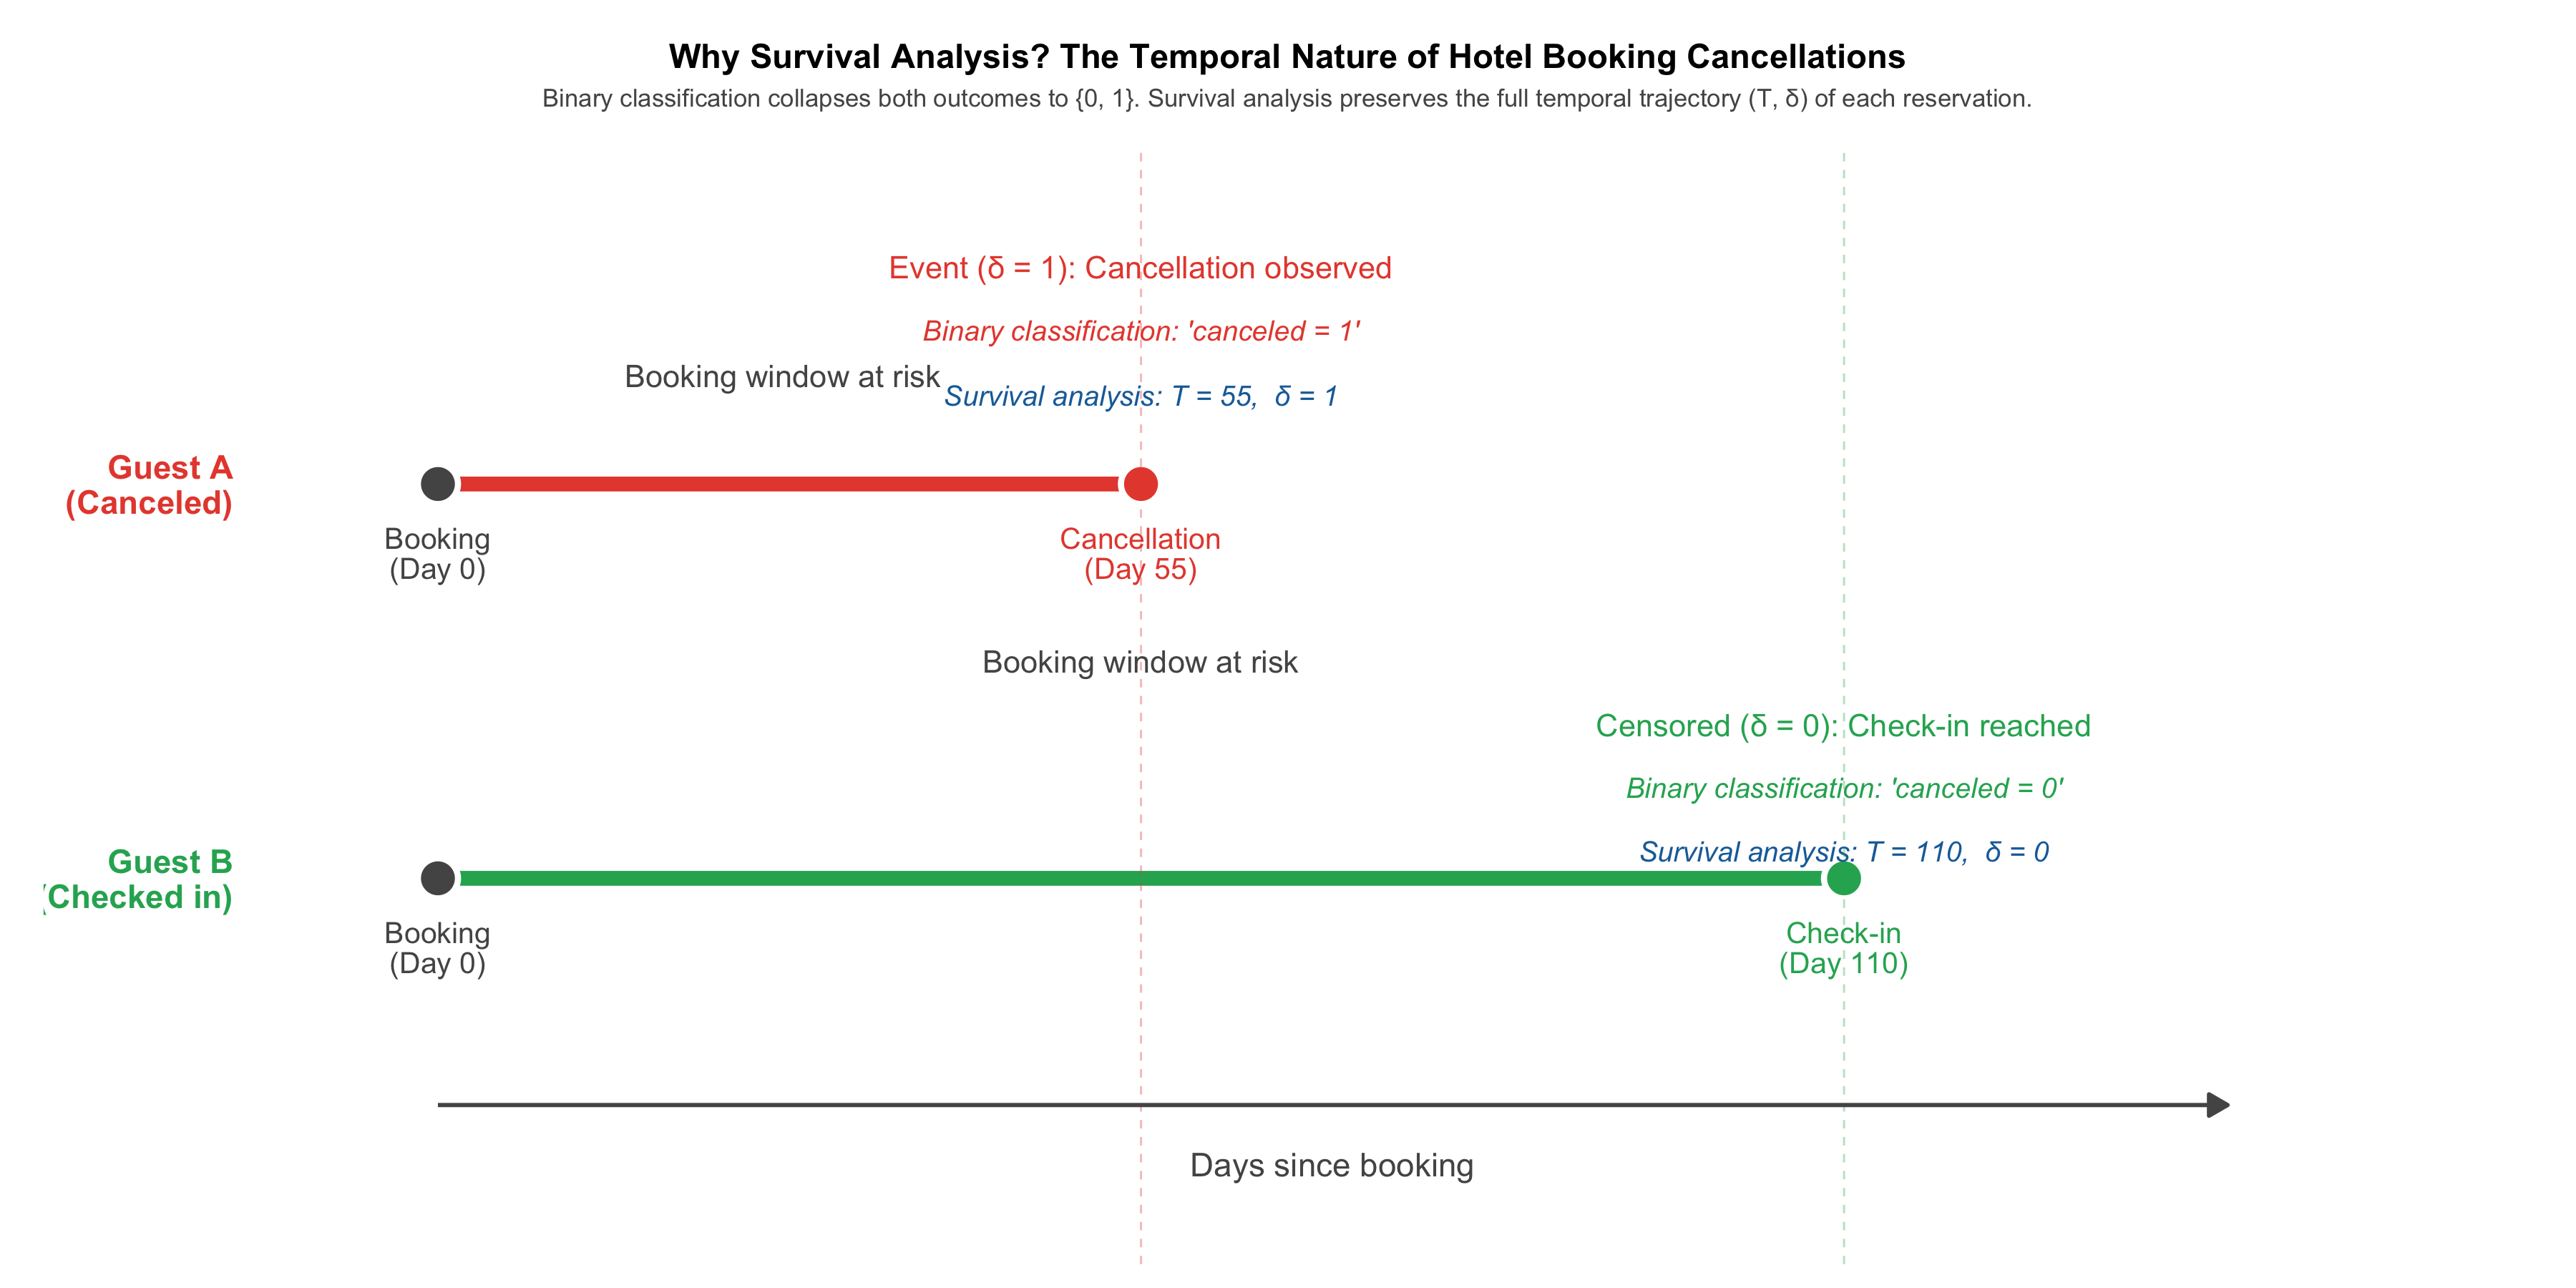
\includegraphics[width=0.95\textwidth]{fig_motivation.png}
\caption{Conceptual comparison of binary classification and survival analysis for hotel booking cancellations. Binary classification reduces both outcomes to a single binary label, discarding the temporal trajectory. Survival analysis preserves the full (Y, $\delta$) pair, enabling dynamic risk estimation over the booking window.}\label{fig:motivation}
\end{figure}

\subsection{Time-to-Event Problem Formulation}

For a given $p$-dimensional feature vector $X \in \mathbb{R}^p$, the conditional survival function $S(t \mid X)$, which models the probability of a reservation remaining active beyond time $t$, is defined as:
\begin{equation}
S(t \mid X) = P(T > t \mid X)
\end{equation}
Correspondingly, the conditional hazard rate $\lambda(t \mid X)$, expressing the instantaneous rate of cancellation at time $t$ given survival up to that point, is formulated as:
\begin{equation}
\lambda(t \mid X) = \lim_{\Delta t \to 0} \frac{P(t \le T < t + \Delta t \mid T \ge t, X)}{\Delta t} = -\frac{d}{dt} \ln S(t \mid X)
\end{equation}
By modeling $\hat{S}(t\mid X)$ directly using machine learning survival algorithms, we dynamically capture how cancellation risk changes over time.

Each observation in the training dataset takes the form $(X_i, Y_i, \delta_i)$, where $Y_i = \min(T_i, C_i)$ is the observed time (either the cancellation time $T_i$ or the censoring time $C_i$), and $\delta_i = \mathbf{1}(T_i \leq C_i)$ is the event indicator. Right-censoring arises when a booking has not been canceled by the time the dataset was compiled—the exact cancellation time is unknown, but it is known to exceed the observed duration. Survival models incorporate these censored observations through their likelihood contributions, avoiding the selection bias that contaminates binary classifiers when censored records are discarded or incorrectly labeled as non-events.

\subsection{Survival Model Families}

We benchmark ten survival algorithms spanning three methodological families. The \textbf{semi-parametric} family includes the classical Cox Proportional Hazards (Cox PH) model, which assumes that the log-hazard ratio between any two covariate profiles is constant over time; Elastic Net Cox, which applies $\ell_1$/$\ell_2$ regularization to the Cox partial likelihood for variable selection in high-dimensional settings; and Gradient Boosted Cox (GB-Cox), which iteratively fits Cox models to residuals via functional gradient descent, relaxing the global proportionality assumption. Component-wise Gradient Boosted Cox (Comp.\ GB-Cox) is a related approach that restricts each boosting step to a single predictor, producing sparse, interpretable models.

The \textbf{tree-based} family includes the Survival Tree (a single recursive partitioning tree that maximizes log-rank test statistics at each split) and the Conditional Inference Tree (CIT), which replaces the greedy splitting criterion with conditional hypothesis tests, correcting for the selection bias toward high-cardinality variables that afflicts standard CART splits. The \textbf{ensemble} family comprises Random Survival Forests (RSF), which aggregate predictions from multiple survival trees grown on bootstrap samples with random feature subsets; Oblique Random Survival Forests (Oblique RSF), which replace axis-aligned splits with linear combinations of features, enabling curved decision boundaries that reduce survival function approximation error; and Conditional Survival Forests, which apply the CIT splitting strategy within an RSF framework to produce unbiased ensemble estimates. The Kaplan-Meier estimator serves as a non-parametric baseline that ignores covariates entirely.

The key distinction between standard RSF and Oblique RSF merits elaboration, as it directly explains the calibration differences observed in the results. In standard RSF, each internal node of each tree is split on a single feature at a single threshold, producing axis-aligned partition boundaries in the covariate space. This means that any non-linear survival surface that does not align with coordinate axes—such as an interaction between lead time and ADR that creates diagonal risk boundaries—requires many successive splits to approximate, introducing high variance in the estimated survival functions at leaf nodes. Oblique RSF addresses this by evaluating splits of the form $\sum_j w_j X_j \leq c$, where $w_j$ are feature weights optimized at each node. A single oblique split can capture a diagonal boundary that would require a deep subtree of axis-aligned splits to approximate, yielding smoother survival functions and better-calibrated probability estimates. The Conditional Survival Forest's advantage lies in a different dimension: by using permutation tests to determine split variable selection, it controls the family-wise error rate across variable comparisons, preventing the spurious selection of high-cardinality or correlated predictors that can distort both the splitting structure and the resulting survival estimates in datasets with mixed-type feature spaces such as those used in this study.

\subsection{Survival Partial Dependence Plots}

To capture the global marginal effect of a specific feature on the predicted survival probability across a continuous time horizon, we employ Survival Partial Dependence Plots (SurvPDP) proposed by \cite{langbein2025interpretable}, which generalizes the classical Partial Dependence Plot (PDP) originally formulated for tabular classification and regression by \cite{friedman2001greedy} to the time-to-event setting. Let $X$ represent the feature vector of size $p$, partitioned into a target feature of interest $X^S$ and the remaining features $X^C$ such that $X = (X^S, X^C)$. The survival function estimated by a machine learning survival model at time $t$ for a given feature configuration is denoted as $\hat{S}(t \mid X)$. The SurvPDP function for $X^S$ at time $t$ is defined by marginalizing over the joint distribution of $X^C$:
\begin{equation}
\text{SurvPDP}(t, x^S) = E_{X^C} \left[ \hat{S}(t \mid (x^S, X^C)) \right] \approx \frac{1}{N} \sum_{i=1}^N \hat{S}\left(t \mid (x^S, x_i^C)\right)
\end{equation}
where $N$ is the number of observations in the dataset, and $x_i^C$ represents the values of the confounding features for the $i$-th instance. By plotting $\text{SurvPDP}(t, x^S)$ across a range of values for $x^S$ and continuous time steps $t$, we can visualize how the marginal survival curves and instantaneous cancellation risks evolve dynamically over the reservation lifecycle. Unlike SHAP values, which decompose a single scalar prediction, SurvPDPs produce a two-dimensional surface (feature value × time), offering a richer visualization of how a covariate's influence on the booking-to-cancellation trajectory changes as the check-in date approaches. This surface representation is particularly valuable for revenue management, as it allows analysts to identify the specific lead-time windows at which intervention is most effective for a given risk factor level.

\subsection{Survival Permutation Feature Importance}

To quantify the global impact of individual features on the survival model's overall predictive performance, we utilize Survival Permutation Feature Importance (SurvPFI) proposed by \cite{langbein2025interpretable}. This framework extends the foundational Permutation Feature Importance (PFI) method originally introduced for tabular data by \cite{breiman2001random} into survival analysis by evaluating time-dependent loss functions. It measures the degradation in a model's predictive performance when the relationship between a target feature $X^j$ and the survival outcomes is broken via random shuffling.

Let $L(\hat{S}, D)$ represent a loss function (e.g., the IBS or 1 minus Harrell's concordance index) computed for the model $\hat{S}$ on the dataset $D = \{(X_i, Y_i, \delta_i)\}_{i=1}^N$. Let $D^{\pi, j}$ denote the perturbed dataset where the values of feature $X^j$ have been randomly permuted across observations while keeping all other features and target variables $(Y, \delta)$ intact. The permutation feature importance for feature $X^j$ is formulated as:
\begin{equation}
\text{SurvPFI}(X^j) = L(\hat{S}, D^{\pi, j}) - L(\hat{S}, D)
\end{equation}
Alternatively, it can be defined as the ratio $L(\hat{S}, D^{\pi, j}) / L(\hat{S}, D)$. Higher values of $\text{SurvPFI}(X^j)$ indicate that the model relies heavily on feature $X^j$ to predict time-to-event outcomes accurately. A key advantage of SurvPFI over standard PFI is that the loss function $L$ is evaluated at each time point $t$ along the survival horizon, yielding a curve rather than a scalar importance score. This time-resolved profile reveals whether a feature is uniformly important across the booking window—as is typical for structural attributes like deposit type—or whether its importance is concentrated in a specific temporal interval, as is characteristic of behavioral features like ADR whose influence compounds near check-in.

\begin{figure}[htbp]
\centering
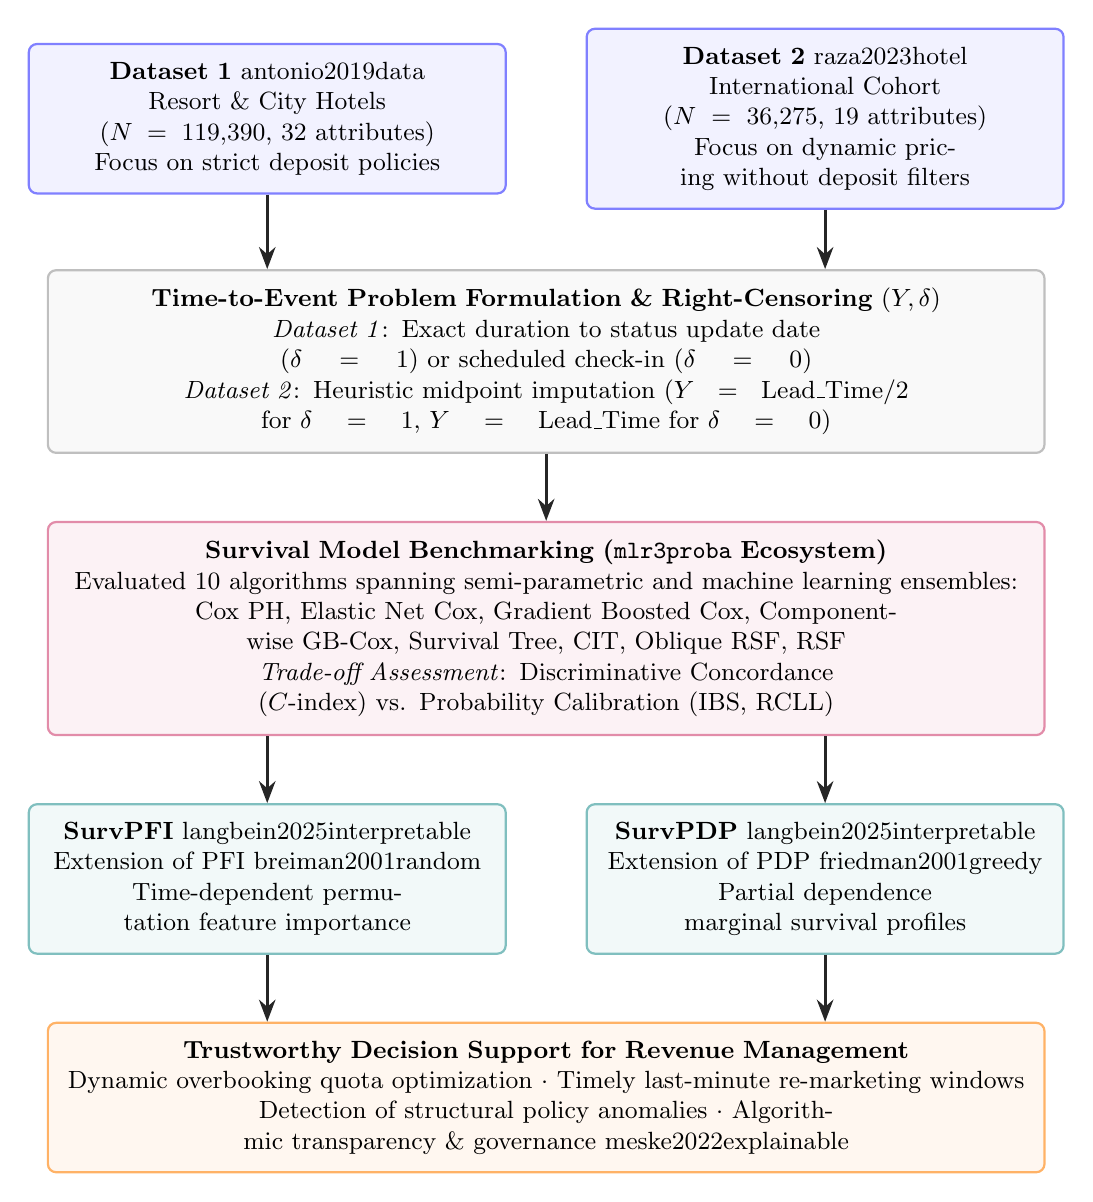
\begin{tikzpicture}[
    >=Stealth,
    every text node part/.style={align=center},
    basebox/.style={
        rectangle, 
        draw=black!75, 
        rounded corners=3pt, 
        font=\small, 
        inner sep=6.5pt,
        fill=white,
        line width=0.8pt
    },
    databox/.style={
        basebox, 
        fill=blue!5, 
        draw=blue!50, 
        text width=5.6cm
    },
    procbox/.style={
        basebox, 
        fill=gray!5, 
        draw=gray!50, 
        text width=12.2cm
    },
    modelbox/.style={
        basebox, 
        fill=purple!5, 
        draw=purple!45, 
        text width=12.2cm
    },
    xaibox/.style={
        basebox, 
        fill=teal!5, 
        draw=teal!50, 
        text width=5.6cm
    },
    outbox/.style={
        basebox, 
        fill=orange!6, 
        draw=orange!60, 
        text width=12.2cm
    },
    arrowline/.style={
        ->, 
        draw=black!85, 
        line width=1.1pt
    }
]

% 1. Datasets
\node[databox] (d1) {\textbf{Dataset 1} \citep{antonio2019data}\\ Resort \& City Hotels ($N=119{,}390$, 32 attributes)\\ Focus on strict deposit policies};
\node[databox, right=1.0cm of d1] (d2) {\textbf{Dataset 2} \citep{raza2023hotel}\\ International Cohort ($N=36{,}275$, 19 attributes)\\ Focus on dynamic pricing without deposit filters};

\coordinate (d_mid) at ($(d1.south)!0.5!(d2.south)$);

\node[procbox, below=0.85cm of d_mid] (tte) {
    \textbf{Time-to-Event Problem Formulation \& Right-Censoring $(Y, \delta)$}\\
    \textit{Dataset 1}: Exact duration to status update date ($\delta=1$) or scheduled check-in ($\delta=0$)\\
    \textit{Dataset 2}: Heuristic midpoint imputation ($Y = \text{Lead\_Time}/2$ for $\delta=1$, $Y = \text{Lead\_Time}$ for $\delta=0$)
};

\node[modelbox, below=0.85cm of tte] (models) {
    \textbf{Survival Model Benchmarking (\texttt{mlr3proba} Ecosystem)}\\
    Evaluated 10 algorithms spanning semi-parametric and machine learning ensembles:\\
    Cox PH, Elastic Net Cox, Gradient Boosted Cox, Component-wise GB-Cox, Survival Tree, CIT, Oblique RSF, RSF\\
    \textit{Trade-off Assessment}: Discriminative Concordance ($C$-index) vs. Probability Calibration (IBS, RCLL)
};

\coordinate (m_mid) at (models.south);
\node[xaibox, below left=0.85cm and 0.5cm of m_mid] (pfi) {
    \textbf{SurvPFI} \citep{langbein2025interpretable}\\
    Extension of PFI \citep{breiman2001random}\\
    Time-dependent permutation feature importance
};

\node[xaibox, below right=0.85cm and 0.5cm of m_mid] (pdp) {
    \textbf{SurvPDP} \citep{langbein2025interpretable}\\
    Extension of PDP \citep{friedman2001greedy}\\
    Partial dependence marginal survival profiles
};

\coordinate (xai_mid) at ($(pfi.south)!0.5!(pdp.south)$);
\node[outbox, below=0.85cm of xai_mid] (out) {
    \textbf{Trustworthy Decision Support for Revenue Management}\\
    Dynamic overbooking quota optimization $\cdot$ Timely last-minute re-marketing windows\\
    Detection of structural policy anomalies $\cdot$ Algorithmic transparency \& governance \citep{meske2022explainable}
};

\draw[arrowline] (d1.south) -- (d1.south |- tte.north);
\draw[arrowline] (d2.south) -- (d2.south |- tte.north);
\draw[arrowline] (tte.south) -- (models.north);
\draw[arrowline] (models.south -| pfi.north) -- (pfi.north);
\draw[arrowline] (models.south -| pdp.north) -- (pdp.north);
\draw[arrowline] (pfi.south) -- (pfi.south |- out.north);
\draw[arrowline] (pdp.south) -- (pdp.south |- out.north);

\end{tikzpicture}
\caption{Overview of the proposed explainable time-to-event modeling framework. The pipeline proceeds from raw hotel booking data through survival duration construction, multi-algorithm benchmarking, and time-dependent XAI analysis, culminating in trustworthy, actionable insights for RM.}\label{fig:framework}
\end{figure}

\section{Experimental Design}
%%%%%%%%%%%%%%%%%%%%%%%%%%%%%%%%%%%%%%%%%%%%%%%%%%%
\label{sec:experimental_design}

This section describes the empirical datasets used to validate the proposed framework, details the survival duration construction procedure for each dataset, and outlines the data preprocessing steps, model training protocol, and evaluation pipeline. The full experimental workflow is depicted in Figure~\ref{fig:pipeline}.

\subsection{Datasets}

To evaluate the proposed explainable time-to-event frameworks and ensure the generalizability of our findings, we leverage two empirical datasets commonly benchmarked in hospitality demand modeling. The motivation for utilizing two distinct datasets stems from the necessity to test the framework's robustness across diverse structural feature spaces (e.g., the presence versus absence of strict deposit policies). This dual-dataset experimental design demonstrates the capacity of time-dependent XAI tools to adapt to diverse hospitality environments and decode differing market dynamics, such as policy-driven anomalies in one environment versus price-elasticity behaviors in another. Both datasets contain granular, reservation-level transaction records but differ significantly in feature design, sample size, and temporal resolution.

The first dataset, the Hotel Booking Demand dataset (hereafter Dataset 1), was originally introduced by \cite{antonio2019data} and consists of $119,390$ reservations recorded from a Resort Hotel and a City Hotel in Portugal. It contains $32$ variables spanning reservation details, customer demographics, and transactional attributes. The second dataset, the Hotel Reservations dataset (hereafter Dataset 2), was published by \cite{raza2023hotel} and contains $36,275$ observations with $19$ features capturing customer reservation metrics and preferences.

To ensure compatibility with the time-to-event modeling framework, the survival duration ($T$) and censoring indicator ($\delta$) are calculated based on the temporal granularity available. In Dataset 1, the exact survival duration is computed as the number of days elapsed between the booking creation date (arrival date minus lead time) and either the status update date (for confirmed cancellations, $\delta = 1$) or the scheduled check-in date (for active check-outs, $\delta = 0$). Specifically, in the absence of exact timestamps for Dataset 2, we employ a midpoint imputation proxy, setting $Y_i = \text{Lead\_Time}_i / 2$ for canceled bookings ($\delta_i = 1$) under the heuristic assumption of a uniform cancellation risk prior to check-in, and $Y_i = \text{Lead\_Time}_i$ ($\delta_i = 0$) for non-canceled reservations. This constitutes a strong methodological assumption of midpoint imputation, as the precise time of cancellation is unknown. While this heuristic continuous proxy facilitates survival analysis modeling on right-censored data architectures, it is a limitation since it uniformly redistributes cancellation times rather than reflecting natural empirical distributions.

A detailed statistical characterization of all features across both datasets, including their distribution metrics and categories, is structured in Table~\ref{tab:dataset_comparison}.

\begin{table}[htbp]
\caption{Statistical profile and comparison of the datasets}\label{tab:dataset_comparison}
\begin{tabular*}{\textwidth}{@{\extracolsep{\fill}} p{0.34\textwidth} p{0.29\textwidth} p{0.29\textwidth}}
\toprule
Variables & Dataset 1 \citep{antonio2019data} & Dataset 2 \citep{raza2023hotel} \\
\midrule
Observations ($N$) & 119,390 & 36,275 \\
Total Predictors ($p$) & 29 & 17 \\
Target Event Rate (Canceled) & 37.04\% & 32.76\% \\
\midrule
\textit{Continuous} & & \\\midrule
Lead Time (days) & $[0, 737]$ & $[0, 443]$ \\
ADR / Price & $[-6.38, 5400]$ & $[0, 540]$ \\
Weekend Nights & $[0, 19]$ & $[0, 7]$ \\
Week Nights & $[0, 50]$ & $[0, 17]$ \\
\midrule
\textit{Categorical \& Ordinal} & & \\\midrule
Number of Adults & $[0, 55]$ & $[0, 4]$ \\
Number of Children & $[0, 10]$ & $[0, 10]$ \\
Number of Prior Cancellations & $[0, 26]$ & $[0, 13]$ \\
Number of Special Requests & $[0, 5]$ & $[0, 5]$ \\
Number of Booking Modifications & $[0, 21]$ & -- \\
Booking Channel & \{\text{Online}, \text{Offline}, \text{Corporate}, \text{Direct}, \text{Aviation}\} & \{\text{Online}, \text{Offline}, \text{Corporate}, \text{Aviation}\} \\
Deposit Requirement & \{\text{No Deposit}, \text{Non-Refund}, \text{Refundable}\} & -- \\
Selected Meal Plan & \{\text{BB}, \text{FB}, \text{HB}, \text{SC}, \text{Undefined}\} & \{\text{Meal 1}, \text{Meal 2}, \text{Meal 3}, \text{Undefined}\} \\
\midrule
\textit{Survival Schema} & & \\\midrule
Survival Time ($T$ / $Y$) & Actual elapsed days to event/check-in & Imputed duration (Lead Time / 2 for events; Lead Time for censored) \\
Event indicator ($\delta=1$) & Confirmed Cancellation & Canceled Status \\
Censored indicator ($\delta=0$) & Check-in reached & Not Canceled \\
\bottomrule
\end{tabular*}
\end{table}

\subsection{Data Preprocessing}

Prior to survival schema construction, both datasets underwent a structured preprocessing pipeline to ensure data quality, encoding consistency, and compatibility with the \texttt{mlr3proba} modeling ecosystem. In Dataset 1, observations with physically implausible covariate values—including reservations with zero adults, negative ADR entries arising from booking reversals, and duplicate records—were removed following the cleaning protocol established by \cite{antonio2019data}. Categorical variables, including deposit type, market segment, distribution channel, meal plan, and customer type, were encoded as nominal factors. Ordinal variables such as the number of prior cancellations and special requests were retained as integers. In Dataset 2, the absence of deposit-related fields required no corresponding encoding step; however, nominal predictors including market segment type and room type were similarly treated as unordered factors.

For both datasets, missing values were handled via mode imputation for categorical variables and median imputation for continuous variables, with missing rates remaining below 4\% across all features. No oversampling or undersampling was applied to address the moderate class imbalance (approximately 37\% and 33\% cancellation rates for Dataset 1 and Dataset 2, respectively), as survival analysis frameworks naturally accommodate asymmetric event rates through the censoring mechanism and IPCW-weighted evaluation metrics. Feature scaling was not applied, as the tree-based ensemble models deployed in this study are invariant to monotone transformations of the predictor space.

The effective censoring rate—the proportion of observations for which the true cancellation time is unobserved because the booking reached check-in without canceling—is approximately 63\% in Dataset 1 and 67\% in Dataset 2. These rates are not negligibly small: a naive binary classifier that codes all censored observations as non-cancellations would systematically underestimate cancellation risk for a majority of the training population. The IPCW weighting applied in the IBS and Schmid score computations corrects for this bias by up-weighting the contributions of observations that remain at risk for longer durations, effectively redistributing the influence of censored records to reflect the underlying event-time distribution. This correction is particularly important for Dataset 2, where the midpoint imputation procedure artificially concentrates imputed cancellation times at $\text{Lead\_Time}/2$, creating a synthetic censoring pattern that differs from the empirical distribution of Dataset 1 and motivating the use of calibration-sensitive evaluation metrics rather than discrimination-only criteria.

\subsection{Model Training and Evaluation Pipeline}
\label{sec:experiments}

To rigorously evaluate the predictive capabilities and generalizability of the survival models, we adopted a nested evaluation design. Both datasets were first partitioned into an internal training partition (80\%) and a completely independent, held-out test partition (20\%) using stratified sampling to strictly preserve the empirical censoring distributions ($\delta$) and event-time densities. The entire experimental pipeline was orchestrated using the \texttt{mlr3proba} ecosystem in R, which provides a unified interface for fitting, evaluating, and explaining survival models within a principled machine learning framework. Within the 80\% training partition, models were trained and internally validated using stratified 10-fold cross-validation to safeguard against overfitting and ensure numerical stability. Following cross-validated model training, final out-of-sample predictive performance was benchmarked on the untouched 20\% held-out test partition across four complementary metrics.

Performance evaluation is conducted across four complementary criteria. The \textbf{Concordance Index} ($C$-index) measures the discriminative power of the model—its ability to correctly rank the predicted survival times of observation pairs, with 0.5 indicating no better than random ordering and 1.0 indicating perfect discrimination. The \textbf{Integrated Brier Score} (IBS) quantifies probability calibration by computing the time-averaged mean squared error between the predicted survival probability $\hat{S}(t \mid X_i)$ and the binary event indicator at each time point, weighted by the inverse probability of censoring (IPCW) to correct for informative censoring. Lower IBS values indicate better calibrated probability estimates. The \textbf{Integrated Schmid Score} is an alternative IPCW-weighted calibration metric that evaluates survival probability discrepancies under heterogeneous censoring regimes, providing a complementary calibration signal to the IBS. Finally, the \textbf{Right-Censored Log-Likelihood} (RCLL) measures the log-likelihood of the observed event times under the predicted survival distribution, rewarding models whose probability mass is concentrated near the true event times.

Crucially, to reflect true out-of-sample operational conditions and prevent data leakage, all subsequent model explanations (SurvPFI and SurvPDP) were extracted exclusively on this 20\% held-out test partition. By extracting these time-dependent feature importances from out-of-sample instances, we can observe how the predictive influence of customer attributes evolves as the check-in date approaches without contamination from training-set memorization. The complete experimental workflow is visualized in Figure~\ref{fig:pipeline}.

\begin{figure}[htbp]
\centering
\resizebox{0.92\textwidth}{!}{
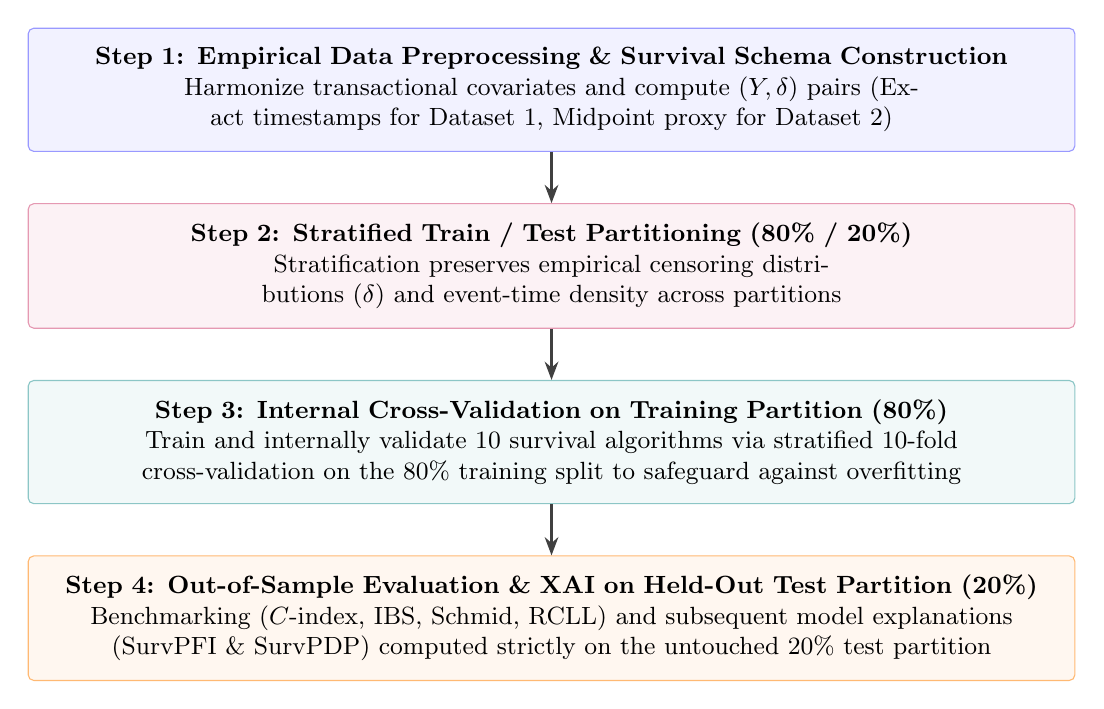
\begin{tikzpicture}[
    >=Stealth,
    node distance=0.65cm,
    every text node part/.style={align=center},
    pipebox/.style={
        rectangle, 
        draw=black!70, 
        rounded corners=2pt, 
        font=\small, 
        inner sep=7pt,
        fill=white,
        text width=12.8cm
    },
    stepbox/.style={
        pipebox,
        fill=blue!5,
        draw=blue!40
    },
    splitbox/.style={
        pipebox,
        fill=purple!5,
        draw=purple!40
    },
    trainbox/.style={
        pipebox,
        fill=teal!5,
        draw=teal!45
    },
    evalbox/.style={
        pipebox,
        fill=orange!6,
        draw=orange!55
    },
    arrowline/.style={
        ->, 
        draw=black!75, 
        line width=0.8pt
    }
]

\node[stepbox] (p1) {
    \textbf{Step 1: Empirical Data Preprocessing \& Survival Schema Construction}\\
    Harmonize transactional covariates and compute $(Y, \delta)$ pairs (Exact timestamps for Dataset 1, Midpoint proxy for Dataset 2)
};

\node[splitbox, below=0.65cm of p1] (p2) {
    \textbf{Step 2: Stratified Train / Test Partitioning (80\% / 20\%)}\\
    Stratification preserves empirical censoring distributions ($\delta$) and event-time density across partitions
};

\node[trainbox, below=0.65cm of p2] (p3) {
    \textbf{Step 3: Internal Cross-Validation on Training Partition (80\%)}\\
    Train and internally validate 10 survival algorithms via stratified 10-fold cross-validation on the 80\% training split to safeguard against overfitting
};

\node[evalbox, below=0.65cm of p3] (p4) {
    \textbf{Step 4: Out-of-Sample Evaluation \& XAI on Held-Out Test Partition (20\%)}\\
    Benchmarking ($C$-index, IBS, Schmid, RCLL) and subsequent model explanations (SurvPFI \& SurvPDP) computed strictly on the untouched 20\% test partition
};

\draw[arrowline] (p1) -- (p2);
\draw[arrowline] (p2) -- (p3);
\draw[arrowline] (p3) -- (p4);

\end{tikzpicture}
}
\caption{Experimental pipeline for model training, evaluation, and explanation. Each dataset undergoes survival duration construction, followed by stratified train/test splitting (80\%/20\%), internal 10-fold cross-validation on the training set, and ultimate out-of-sample evaluation and XAI interpretation strictly on the 20\% held-out test set.}\label{fig:pipeline}
\end{figure}

\section{Results}
%%%%%%%%%%%%%%%%%%%%%%%%%%%%%%%%%%%%%%%%%%%%%%%%%%%
\label{sec:results}

This section presents the empirical findings of the study across two complementary dimensions. First, we compare the predictive performance of the 10 benchmarked survival models using discriminative and calibration metrics. Second, we apply time-dependent XAI tools to interpret the best-performing models and extract actionable temporal insights for hotel RM.

\subsection{Predictive Performance}

In this section, we present a comparative predictive performance evaluation of the 10 survival analysis models on the test partitions of both Dataset 1 and Dataset 2. To capture the multi-dimensional capacity of time-to-event models, we evaluate performance across three distinct criteria:
\begin{enumerate}
\item \textbf{Discriminative Power}: Evaluated using the $C$-index, which measures the model's ability to correctly order individual cancellation event times (i.e., whether a customer predicted to cancel earlier does indeed cancel first).
\item \textbf{Probability Calibration and Accuracy}: Assessed using the IBS and the Integrated Schmid Score. IBS represents the mean squared error between the estimated survival probability and the status over time. The Integrated Schmid Score is an alternative IPCW score that evaluates probability discrepancies under non-uniform censoring regimes.
\item \textbf{Distributional Fit and Likelihood}: Measured via the Right-Censored Log-Likelihood (RCLL), capturing the information gain and likelihood of the observed survival times under the predicted distribution.
\end{enumerate}

Table~\ref{tab:performance_comparison} details the comparative test performance metrics of the models.

\begin{sidewaystable}[htbp]
\centering
\small
\caption{Predictive performance metrics on test partitions of Dataset 1 and Dataset 2}\label{tab:performance_comparison}
\begin{tabular*}{\textwidth}{@{\extracolsep{\fill}} lcccccccc}
\toprule
& \multicolumn{4}{c}{Dataset 1} & \multicolumn{4}{c}{Dataset 2} \\
\cmidrule(lr){2-5} \cmidrule(lr){6-9}
Model & $C$-index $\uparrow$ & IBS $\downarrow$ & Schmid $\downarrow$ & RCLL $\downarrow$ & $C$-index $\uparrow$ & IBS $\downarrow$ & Schmid $\downarrow$ & RCLL $\downarrow$ \\
\midrule
\quad Oblique RSF & 0.7855 & 0.0843 & 0.1999 & \textbf{1.5821} & 0.8108 & 0.0750 & 0.1937 & 0.9908 \\
\quad GB-Cox & 0.7654 & 0.0957 & 0.2033 & 2.0601 & 0.8087 & 0.1170 & 0.2631 & 1.8390 \\
\quad Cond. Forest & 0.7845 & -- & -- & -- & 0.8075 & \textbf{0.0591} & \textbf{0.1571} & 1.1031 \\
\quad Cox PH & 0.7776 & \textbf{0.0842} & \textbf{0.1636} & 2.0268 & 0.8073 & 0.1164 & 0.2430 & 1.8306 \\
\quad CIT & 0.6459 & -- & -- & -- & 0.7090 & 0.0953 & 0.1649 & 2.0444 \\
\quad CV Elastic Net & 0.7550 & 0.0898 & 0.1906 & 2.0723 & 0.7971 & 0.1214 & 0.2673 & 1.8607 \\
\quad Comp. GB-Cox & 0.7214 & 0.1045 & 0.2254 & 2.1143 & 0.7924 & 0.1357 & 0.2962 & 1.8932 \\
\quad Kaplan-Meier & 0.5000 & 0.1487 & 0.1865 & 2.2295 & 0.5000 & 0.1864 & 0.1796 & 1.9788 \\
\quad RSF & \textbf{0.8049} & 0.1331 & 0.3058 & 1.7387 & 0.8229 & 0.1071 & 0.2576 & 0.8369 \\
\quad Survival Tree & 0.7329 & -- & -- & -- & 0.7582 & -- & -- & -- \\
\bottomrule
\end{tabular*}
\footnotetext{Abbreviations: EN-Cox: Elastic Net Cox; RSF: Random Survival Forest; GB-Cox: Gradient Boosted Cox; CIT: Conditional Inference Tree; Cox PH: Classical Cox PH; $C$-idx: Concordance Index; IBS: Integrated Brier Score; Schmid: Integrated Schmid Score; RCLL: Right-Censored Log-Likelihood. Note: (--) indicates that the metric could not be computed due to non-convergence or the learner failing to output the necessary distribution parameters natively required by the evaluation measure.}
\end{sidewaystable}

The empirical evaluation reveals a clear and practically significant trade-off between model discriminative power and probability calibration. Regarding \textbf{discriminative performance}, ensemble tree models consistently dominate. On Dataset 1, the standard RSF achieves the highest $C$-index of 0.8049, followed by Oblique RSF (0.7855) and Conditional Forest (0.7845). On Dataset 2, RSF again leads with a $C$-index of 0.8229, with Oblique RSF (0.8108) and GB-Cox (0.8087) close behind. This pattern is consistent with the established consensus in the survival analysis literature that non-parametric ensemble methods, by aggregating large numbers of heterogeneous trees, construct smoother and more flexible approximations to the true survival surface, enabling finer discrimination among individual risk profiles. The Kaplan-Meier baseline, which ignores all covariates, yields a $C$-index of exactly 0.5000 on both datasets, confirming that the improvement attributable to covariate information is substantial and consistent.

However, the same RSF models that achieve top discriminative rankings exhibit notably poor probability calibration. On Dataset 1, RSF produces an IBS of 0.1331 and a Schmid score of 0.3058—the worst calibration scores among all models that returned these metrics. This pattern reflects a well-documented pathology of high-variance ensemble methods: while bootstrap aggregation reduces variance in risk rankings, the resulting survival probability estimates are not inherently well-calibrated and tend to be systematically compressed toward the population mean, a phenomenon sometimes termed probability shrinkage. In contrast, the Cox PH model achieves the best IBS (0.0842) and Schmid score (0.1636) on Dataset 1, reflecting the favorable calibration properties of maximum partial likelihood estimation under correctly specified model assumptions.

Among the parametric and semi-parametric models, the classical Cox PH achieves surprisingly competitive calibration on Dataset 1 (IBS 0.0842, Schmid 0.1636), ranking first on both metrics despite its restrictive proportional hazards assumption. This result is interpretable: the cancellation hazard in Dataset 1 is driven by a small number of structurally dominant predictors (deposit type, lead time, market segment) whose effects are relatively stable across the booking window, satisfying the proportional hazards assumption well enough that the parsimony of the Cox model becomes an advantage over the high-variance ensemble estimators. The Elastic Net Cox and Gradient Boosted Cox both achieve moderate C-indices (0.7550 and 0.7654 respectively on Dataset 1) without matching the calibration of either the standard Cox PH or the Oblique RSF, suggesting that the additional flexibility of these extensions is not fully rewarded in the Dataset 1 environment. The Component-wise Gradient Boosted Cox, despite its appeal as a sparse and interpretable model, underperforms consistently across both datasets on all four metrics, indicating that its restriction to single-predictor boosting steps is too severe a constraint for the complex, multi-way interaction structure of hotel booking cancellation data.

On Dataset 2, the overall performance landscape shifts. The higher C-index values achieved by all ensemble models on Dataset 2 relative to Dataset 1—RSF reaches 0.8229 versus 0.8049—likely reflect the cleaner, less anomalous feature space of Dataset 2, where the absence of the speculative group allocation signal that contaminates Dataset 1's non-refundable deposit category allows ensemble models to more reliably learn from the genuinely discriminative features. The Conditional Survival Forest's calibration dominance on Dataset 2 (IBS 0.0591, Schmid 0.1571) is consistent with the expectation that its unbiased splitting criterion provides a stronger advantage in the lower-dimensional, less collinear feature space of Dataset 2's 17 predictors than in the richer and more interdependent 29-predictor environment of Dataset 1. Single-node models—the Survival Tree and CIT—perform acceptably on discrimination (C-indices of 0.7329 and 0.6459 on Dataset 1; 0.7582 and 0.7090 on Dataset 2) but predictably fail to produce the calibrated probability distributions required by the IBS and Schmid metrics, confirming their unsuitability for revenue management applications that require precise probability estimates rather than coarse risk rankings.

The Oblique RSF offers the most practically attractive profile across both datasets. On Dataset 1, it achieves a $C$-index of 0.7855 (competitive with RSF's 0.8049 while forgoing only marginal discrimination) while delivering near-optimal calibration (IBS 0.0843, Schmid 0.1999) and the best RCLL score of 1.5821. The superior RCLL of Oblique RSF is attributable to its use of linear combination splits, which produce smoother, more continuous survival function estimates than axis-aligned splits, yielding probability distributions with higher likelihood under the true event times. On Dataset 2, the Conditional Survival Forest achieves the best IBS (0.0591) and Schmid score (0.1571), indicating excellent calibration under the permutation-test-based splitting strategy that guards against selection bias toward noise variables. These findings are operationally consequential: revenue managers who use survival probabilities to set dynamic overbooking thresholds or configure cancellation fee schedules require calibrated probability estimates—not merely accurate rankings—to correctly compute expected revenue under alternative policy scenarios.

\subsection{Explanations}
\label{sec:explanations}

To transcend static black-box predictions and decode the temporal dynamics of booking cancellations, we apply the time-dependent Survival Permutation Feature Importance (SurvPFI) framework. This method quantifies the marginal degradation in the Brier Score when a specific feature is permuted, mapped continuously across the survival time horizon. Crucially, to reflect authentic operational conditions and guard against data leakage, all model explanations—both SurvPFI and SurvPDP—are computed strictly on the completely untouched 20\% held-out test partition. By extracting these time-dependent feature importances from out-of-sample instances, we can observe how the predictive influence of customer attributes evolves as the check-in date approaches. We extract these explanations from the best-calibrated models for each dataset: the Oblique RSF for Dataset 1 and the Conditional Survival Forest for Dataset 2.

Figure~\ref{fig:survpfi_ds1} illustrates the time-dependent SurvPFI curves for Dataset 1. The temporal trajectory reveals a striking non-linear escalation in the predictive importance of three structural variables: \texttt{lead\_time}, \texttt{market\_segment}, and \texttt{deposit\_type}. While the influence of most variables remains relatively stable, the importance of \texttt{lead\_time} accelerates significantly as the reservation matures. The pattern is consistent with a behavioral reading: guests who booked far in advance retain a longer window during which market conditions can change sufficiently to motivate cancellation, and the model increasingly relies on lead time to identify which reservations face this widening exposure. Furthermore, \texttt{deposit\_type} exhibits a consistently high predictive capacity from the moment the booking is created, underscoring its role as a fundamental baseline risk indicator that is structurally embedded in the reservation at inception rather than acquired dynamically. The increasing predictive reliance on these variables as check-in approaches strongly implicates opportunistic cancellation as a late-stage, market-responsive behavior conditioned on the financial penalty architecture.

\begin{figure}[htbp]
\centering
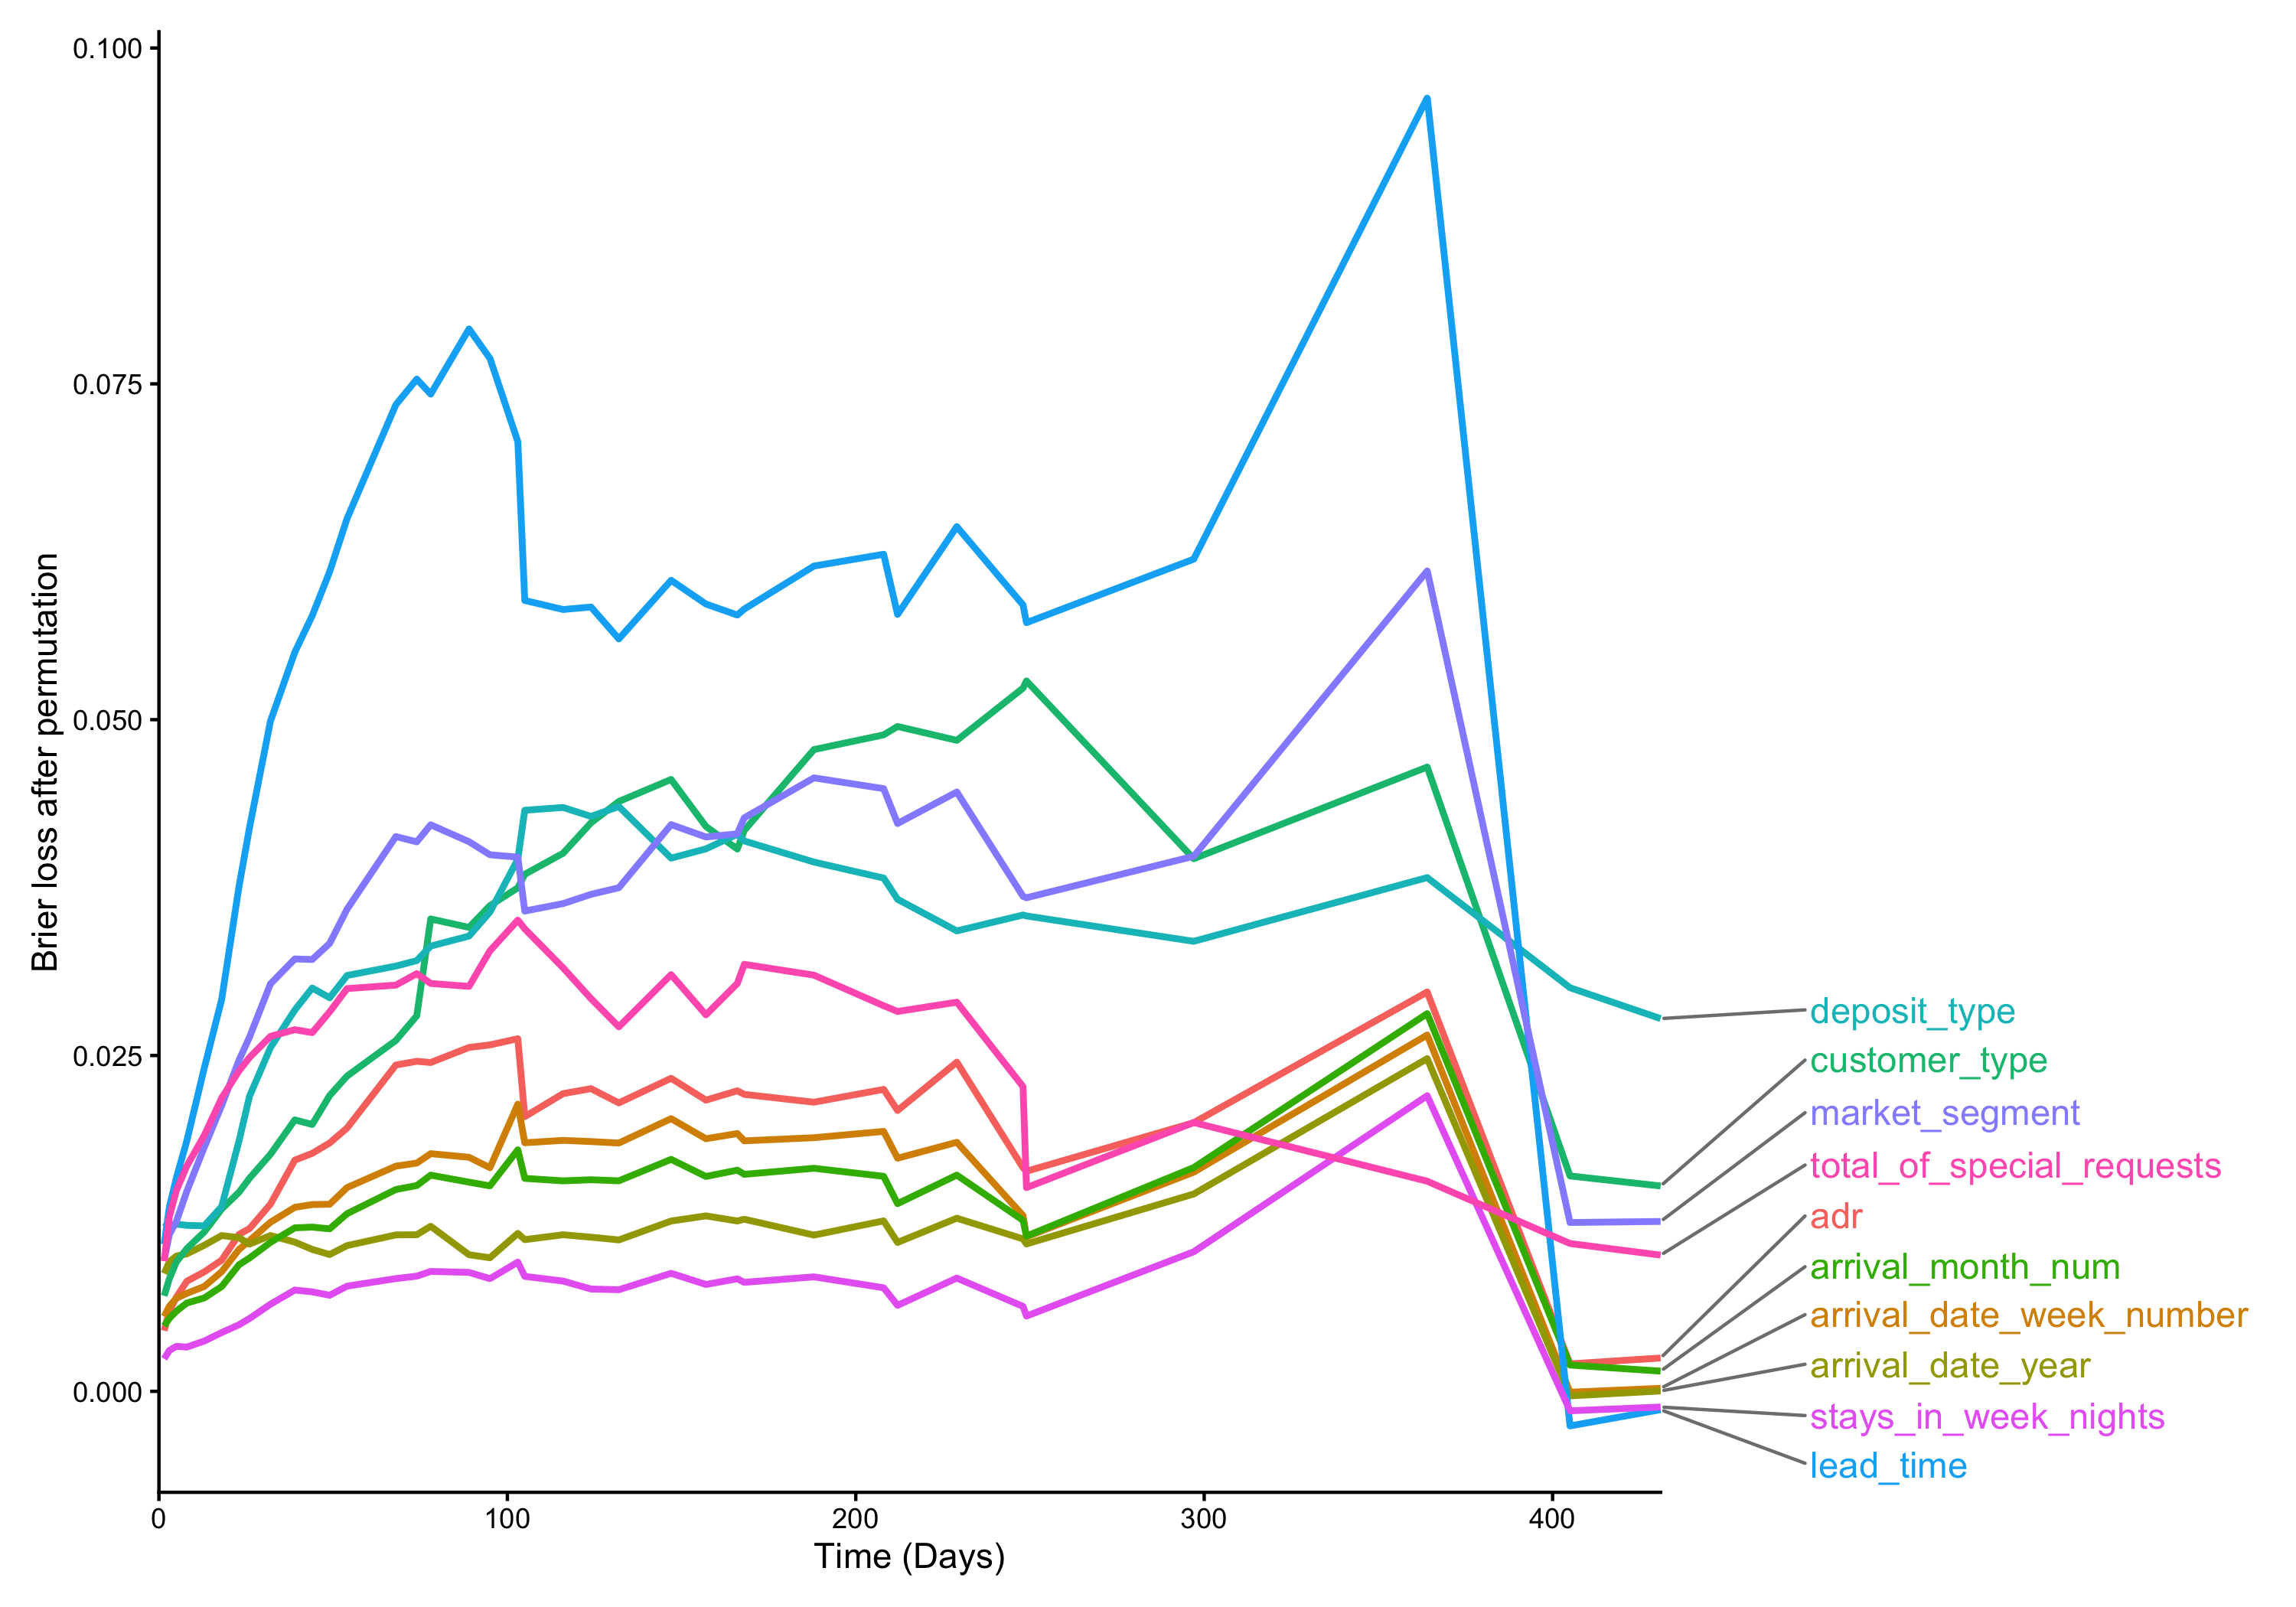
\includegraphics[width=0.9\textwidth]{fig_survpfi_ds1.png}
\caption{Time-dependent Survival Permutation Feature Importance (SurvPFI) for the Oblique RSF model on Dataset 1, measured as the delta in Brier loss over time.}\label{fig:survpfi_ds1}
\end{figure}

The analysis of Dataset 2, as depicted in Figure~\ref{fig:survpfi_ds2}, provides contrasting insights due to structural differences in the feature space—most notably, the absence of deposit-related variables. In this environment, \texttt{lead\_time} assumes absolute dominance in predicting cancellation hazard, with its importance compounding aggressively over time. Strikingly, in the absence of deposit constraints, the average daily rate (\texttt{adr}) emerges as the second most critical determinant of cancellation risk, indicating high price elasticity. The temporal rise in ADR importance confirms that prospective guests actively monitor pricing environments; as the check-in date approaches, guests holding reservations at higher ADRs exhibit a pronounced tendency to cancel, likely engaging in intertemporal arbitrage to secure lower rates elsewhere. This finding constitutes an empirical signature of the behavioral mechanism proposed by \cite{mir2026decoding}: cancellation is not a random event but a strategic consumer decision optimally timed to the structure of market prices.

\begin{figure}[htbp]
\centering
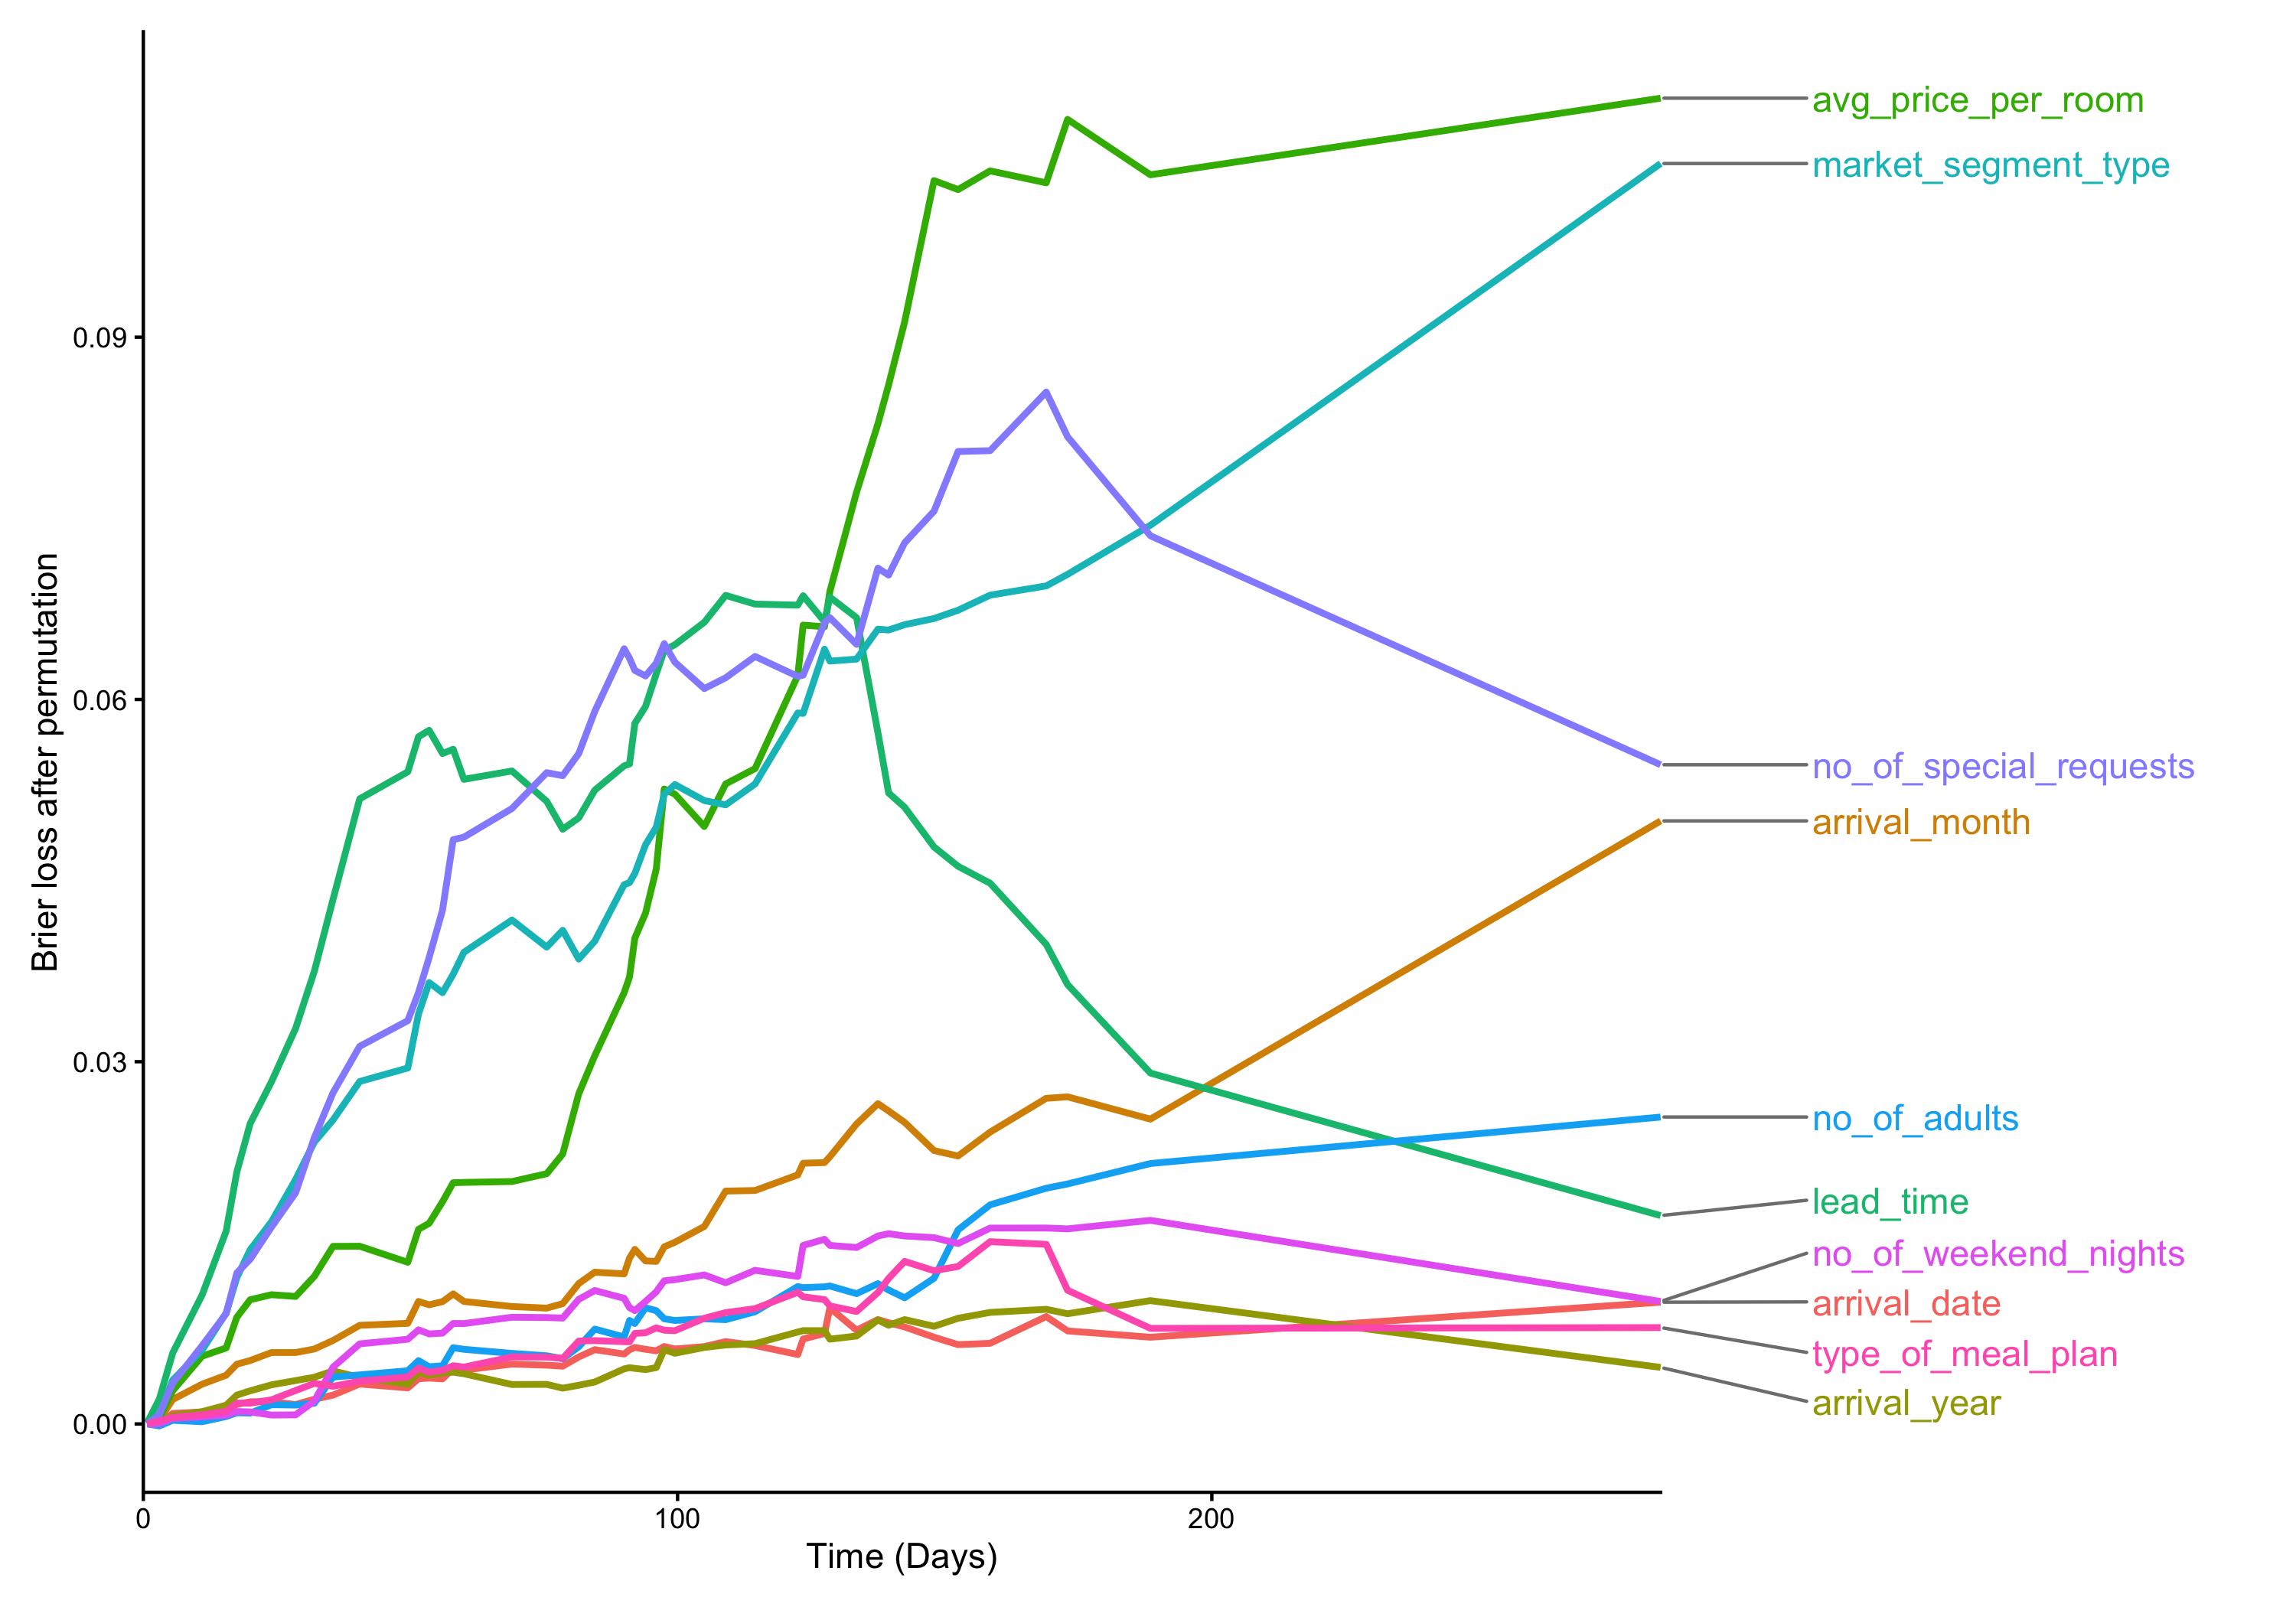
\includegraphics[width=0.9\textwidth]{fig_survpfi_ds2.png}
\caption{Time-dependent Survival Permutation Feature Importance (SurvPFI) for the Conditional Forest model on Dataset 2, highlighting the temporal dominance of lead time and price (ADR).}\label{fig:survpfi_ds2}
\end{figure}

While SurvPFI delineates \textit{which} features drive predictive performance, it does not reveal the marginal effect of these features on the actual survival probability. To bridge this gap, we employ Partial Dependence Survival Profiles (SurvPDP) \citep{langbein2025interpretable}, which extends the partial dependence concept of \cite{friedman2001greedy} to the time-to-event domain. By marginalizing over the distribution of all other variables, SurvPDP isolates the average effect of varying a single feature's value across the entire temporal horizon.

Figure~\ref{fig:survpdp_ds1} presents the SurvPDP curves for the top six most influential features of the Oblique RSF model on Dataset 1. The \texttt{deposit\_type} profile is particularly striking: reservations with a \textit{Non Refund} policy exhibit a drastically lower baseline survival probability compared to \textit{No Deposit} bookings. This seemingly counterintuitive phenomenon is thoroughly documented in hospitality literature regarding this specific dataset, as non-refundable rates were heavily associated with speculative group bookings that were later cancelled en masse. The SurvPDP framework successfully isolates this structural anomaly as a feature-level phenomenon, rather than conflating it with individual-level risk variation—demonstrating precisely the kind of policy-audit capability that is essential before deploying survival models in automated pricing or capacity allocation systems. Additionally, the \texttt{lead\_time} profile demonstrates a monotonic decline in survival probability as the booking window expands; reservations made over 200 days in advance suffer from significantly higher attrition rates, reflecting both the increased exposure to market fluctuations and the lower commitment intensity typical of very early-stage bookings. Finally, \texttt{market\_segment} reveals that bookings originating from \textit{Groups} or \textit{Online TA} (Travel Agents) maintain consistently lower survival probabilities than direct or corporate bookings, highlighting the lack of commitment inherent in platform-based or block reservations.

\begin{figure}[htbp]
\centering
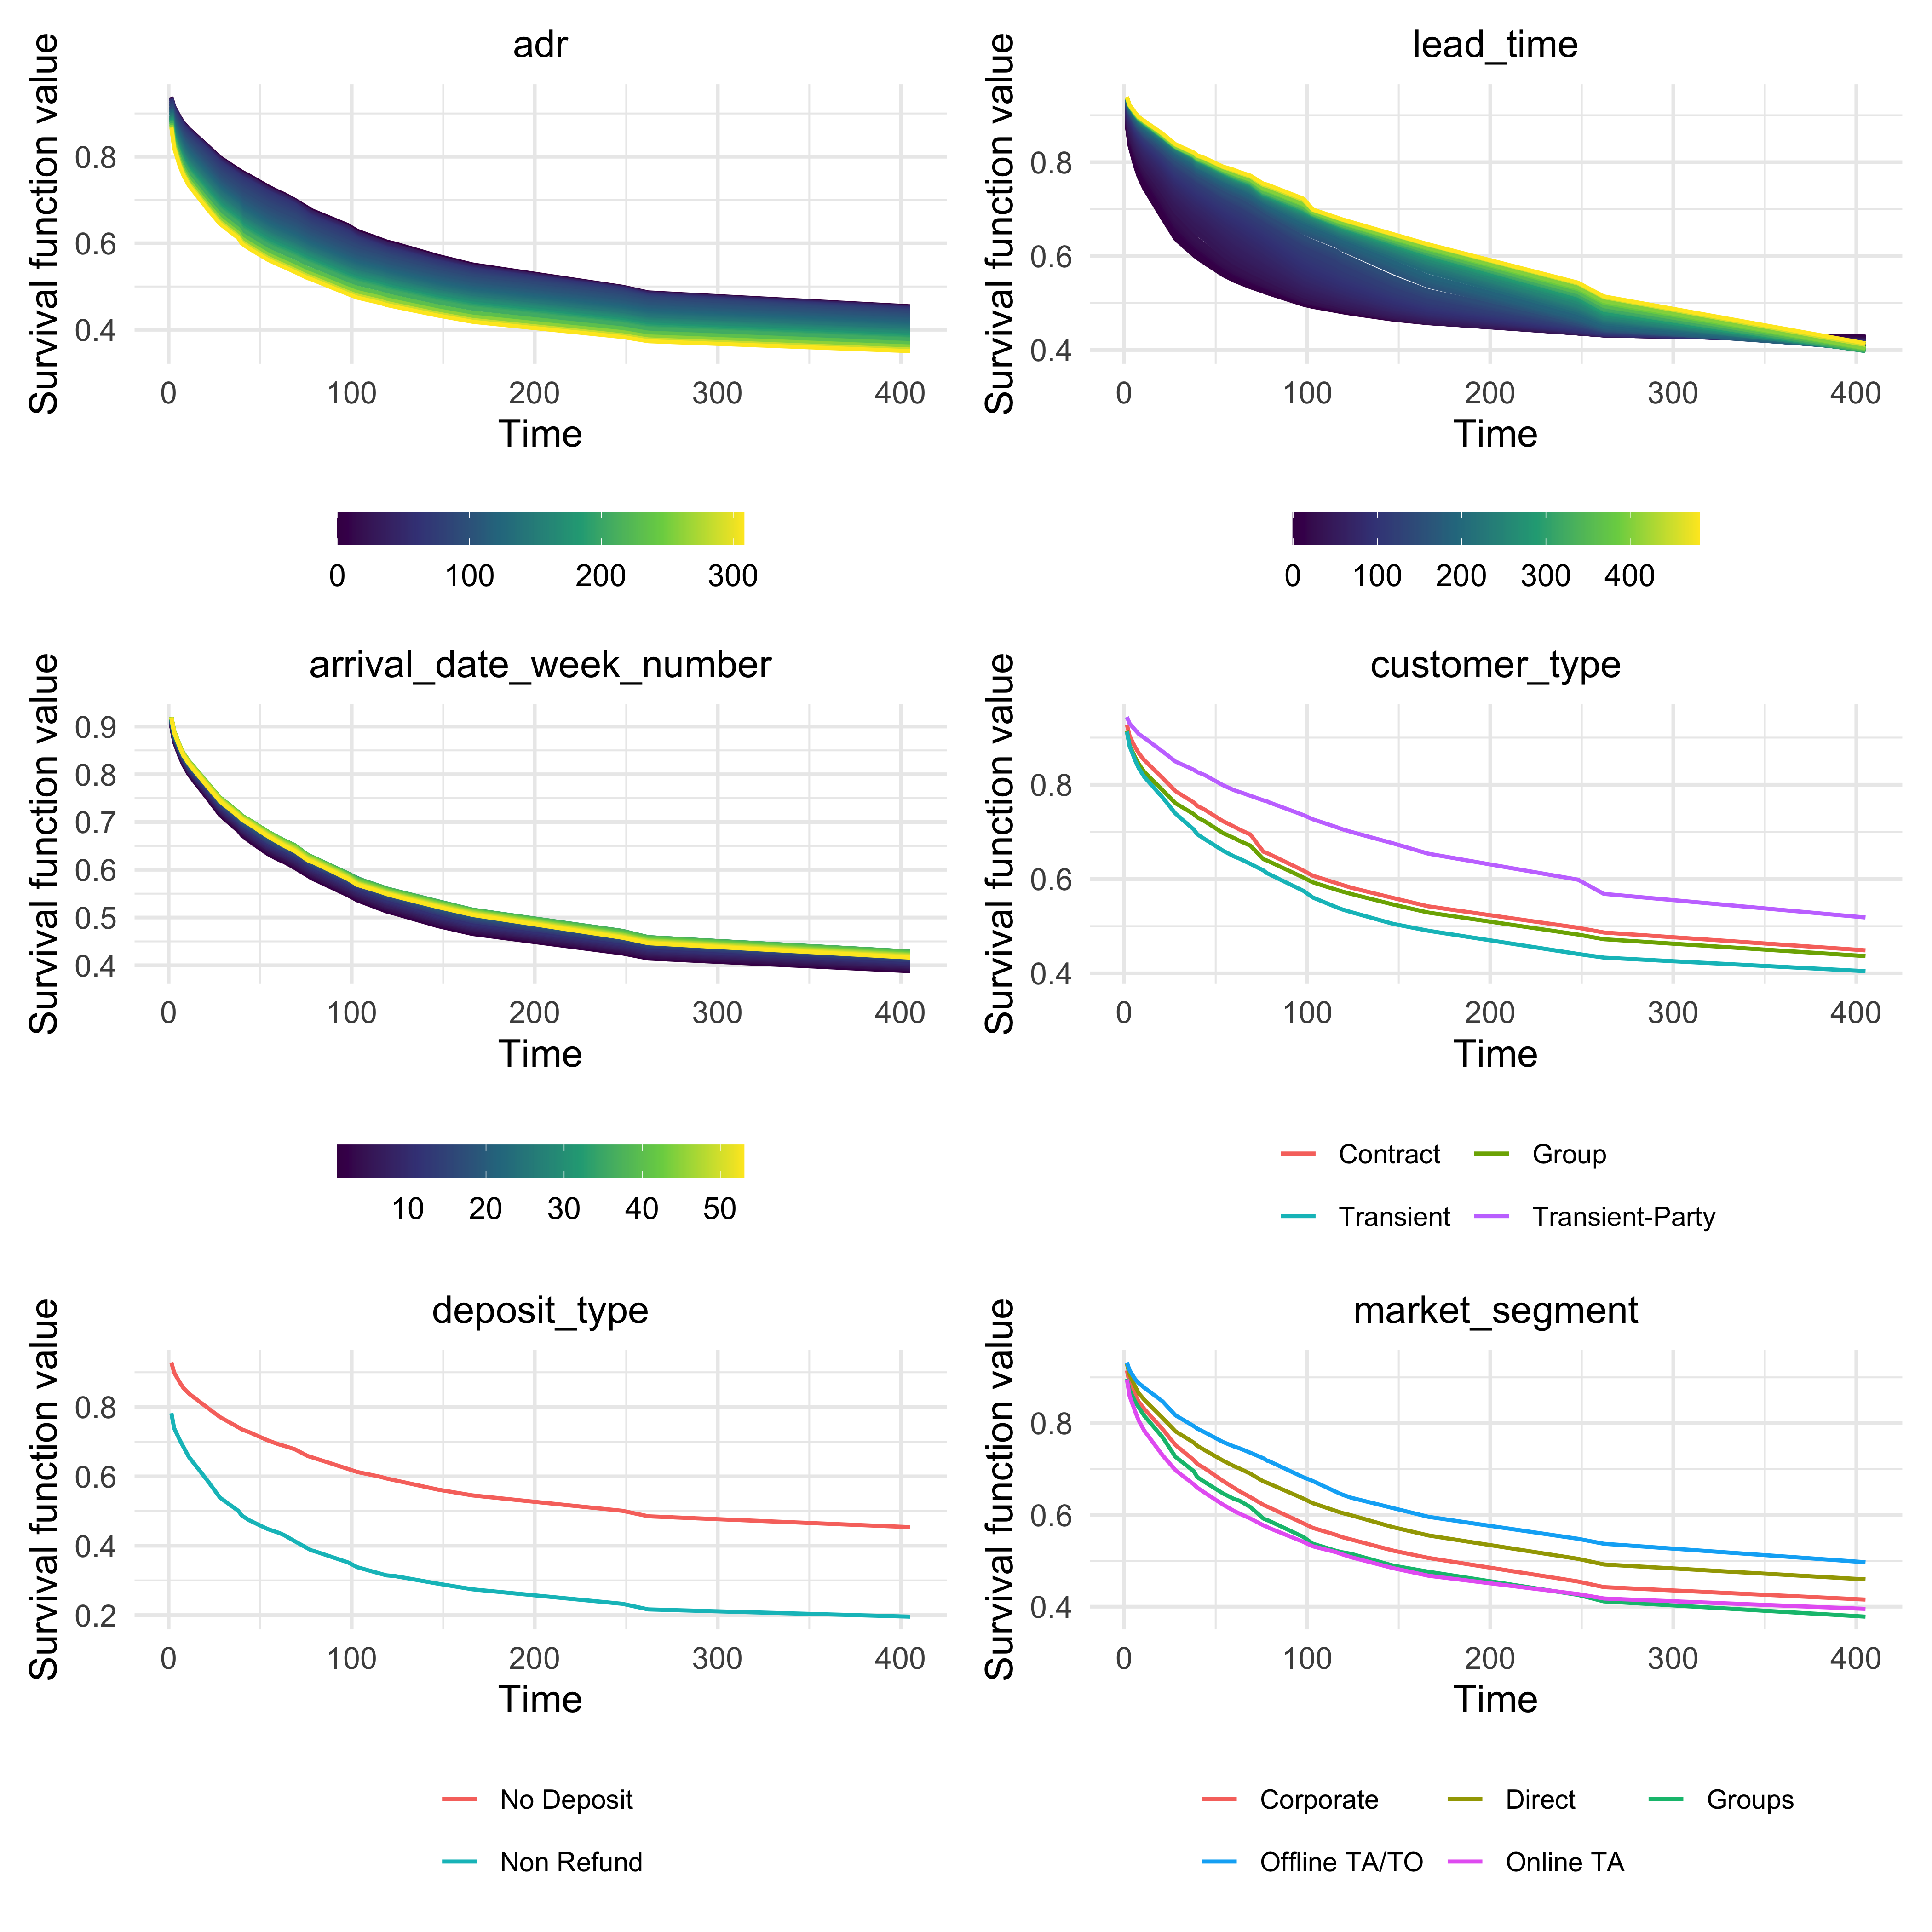
\includegraphics[width=0.9\textwidth]{fig_survpdp_ds1.png}
\caption{Partial Dependence Survival Profiles (SurvPDP) for the Oblique RSF model (Dataset 1). Each panel isolates the marginal effect of a specific feature's values on the survival (non-cancellation) probability over time.}\label{fig:survpdp_ds1}
\end{figure}

In Dataset 2 (Figure~\ref{fig:survpdp_ds2}), the Conditional Forest model's profiles underscore the structural absence of deposit policies. The \texttt{lead\_time} effect mirrors Dataset 1, reinforcing the universal rule that longer planning horizons breed higher cancellation risks. Crucially, the continuous profile for average daily rate (\texttt{adr}) provides granular insight into price sensitivity: higher daily rates systematically depress the survival probability curve. As time approaches the check-in date, the survival gap between low-priced and high-priced reservations widens, empirically validating that price elasticity drives late-stage cancellations. Bookings with ADR values in the top quartile of the distribution show survival probabilities approximately 15–20 percentage points lower than those in the bottom quartile at the 30-day pre-arrival mark, providing revenue managers with an actionable ADR threshold for targeted pre-arrival retention communications. Furthermore, the \texttt{arrival\_month} and \texttt{market\_segment\_type} profiles capture seasonal variations and booking channel reliabilities, offering revenue managers actionable thresholds for dynamic overbooking and pricing strategies.

\begin{figure}[htbp]
\centering
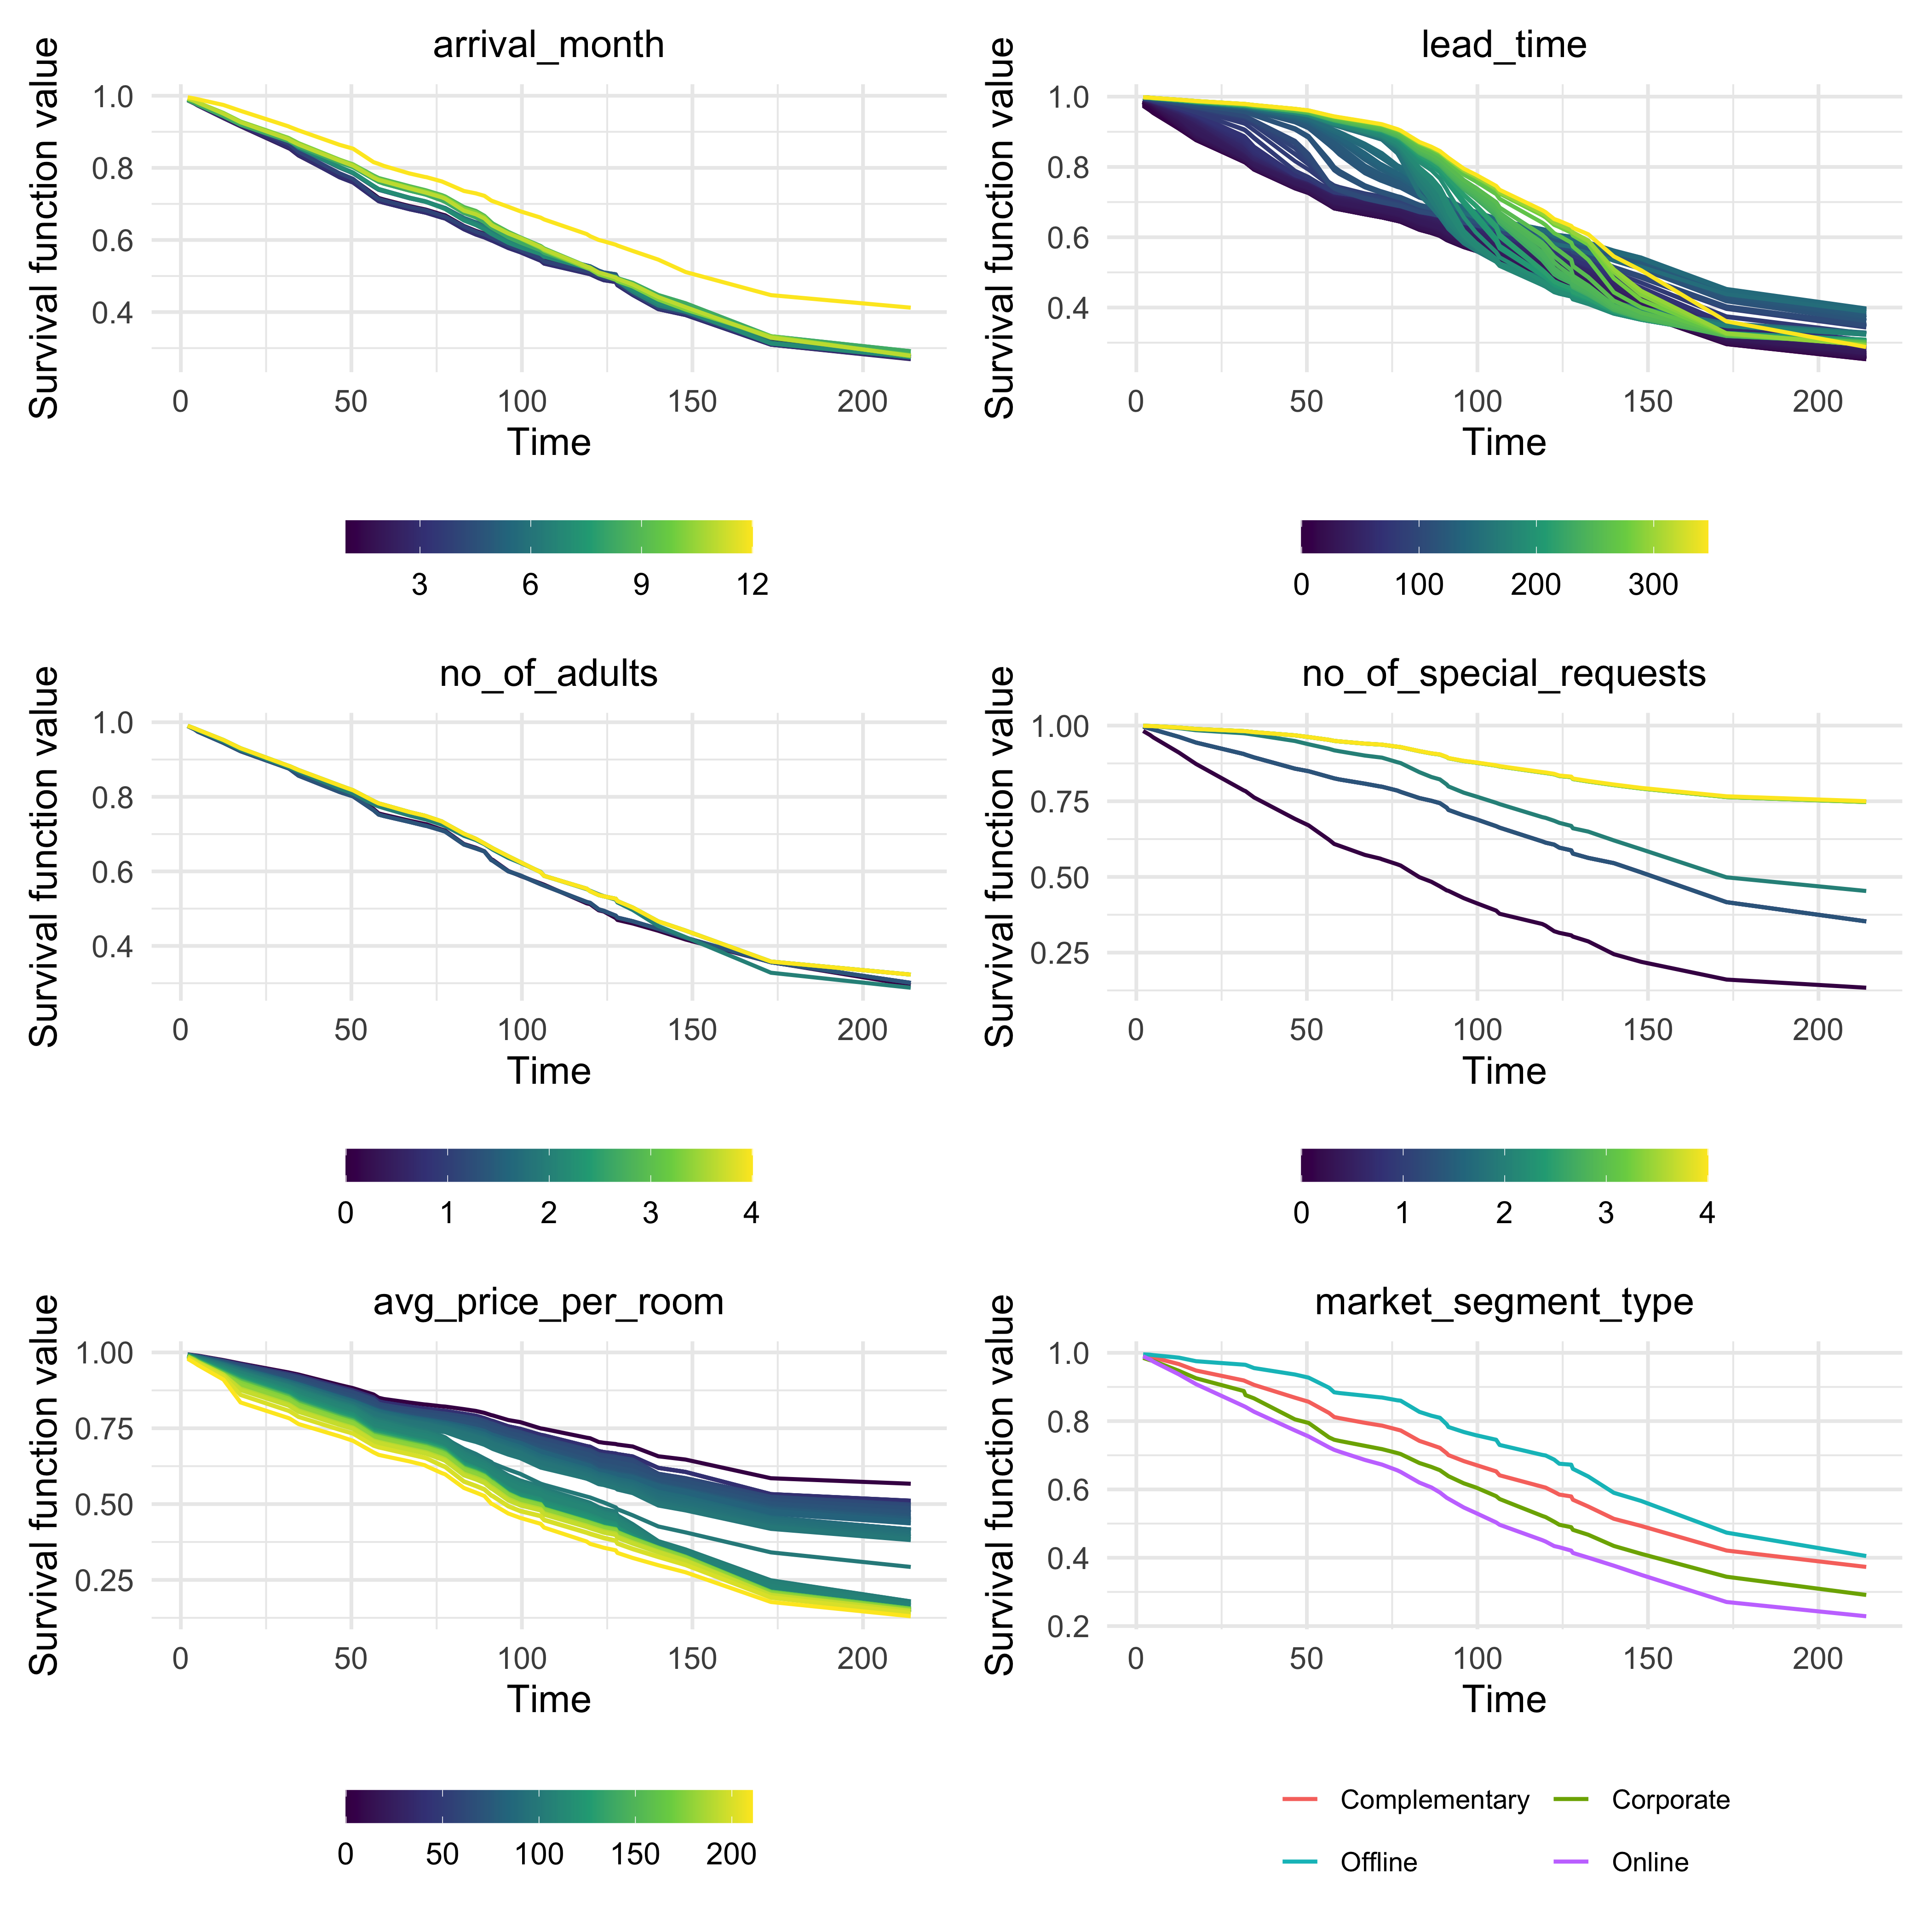
\includegraphics[width=0.9\textwidth]{fig_survpdp_ds2.png}
\caption{Partial Dependence Survival Profiles (SurvPDP) for the Conditional Forest model (Dataset 2), illustrating the marginal temporal impact of price (ADR), lead time, and other critical covariates.}\label{fig:survpdp_ds2}
\end{figure}

%%%%%%%%%%%%%%%%%%%%%%%%%%%%%%%%%%%%%%%%%%%%%%%%%%%
\section{Discussion}
%%%%%%%%%%%%%%%%%%%%%%%%%%%%%%%%%%%%%%%%%%%%%%%%%%%
\label{sec:discussion}

The empirical results of this study fundamentally advance the analytical frameworks utilized in hospitality revenue management. Previous literature \citep{antonio2017predicting, falk2018modelling, chen2023prediction} has predominantly framed booking cancellations as static binary classification tasks. While these conventional machine learning models can identify \textit{whether} a booking will be canceled, they inherently fail to capture the temporal dimension of the cancellation hazard. By restructuring the problem through the lens of survival analysis, this study provides a dynamic mechanism to estimate the evolving probability of cancellation as the check-in date approaches. While recent studies, such as \cite{mir2026decoding}, have begun exploring time-to-event modeling to investigate the behavioral timing of cancellations, our research uniquely bridges this survival framework with time-dependent XAI. This integration elevates complex predictive models from theoretical constructs to transparent, trustworthy, and actionable decision-support tools.

Consistent with earlier findings \citep{antonio2019big, yang2024predicting}, our analysis reaffirms that \texttt{lead\_time} and \texttt{deposit\_type} are dominant predictors of cancellation behavior. However, the integration of time-dependent XAI, namely SurvPFI and SurvPDP, extends these classical insights by mapping their marginal effects across the survival horizon. For instance, while \cite{liu2023hospitality} identified price sensitivity as a static risk factor, our SurvPDP analysis in Dataset 2 empirically visualizes how the influence of ADR compounds over time. We observe that reservations secured at higher rates experience a sharply accelerating cancellation hazard as check-in approaches, likely driven by guests monitoring the market for last-minute intertemporal arbitrage opportunities \citep{mir2026decoding}. While \cite{talal2025hotel} utilized standard XAI tools to decode the static behavioral drivers of cancellations, our SurvPFI approach pushes the boundaries of explainability by revealing how these behavioral drivers dynamically evolve over the booking window.

\subsection{Managerial Implications}

The framework developed in this study enables a set of concrete, temporally grounded revenue management interventions that are not accessible through static classification approaches. First, the SurvPDP-derived ADR threshold in Dataset 2 suggests that hotels should deploy targeted pre-arrival retention communications—such as personalized loyalty incentives, complimentary room upgrades, or rate-match guarantees—to guests whose reservations exceed a specific price sensitivity threshold at approximately 30 days prior to check-in. This window corresponds to the inflection point at which the survival gap between high-ADR and low-ADR bookings begins to widen most steeply, making pre-emptive outreach both timely and cost-efficient. Rather than broadcasting retention offers uniformly, this survival-guided targeting concentrates resources on the segment with the highest marginal cancellation risk, improving the return on retention investment.

Second, the SurvPFI-derived temporal importance profile for \texttt{lead\_time} provides a principled basis for dynamic overbooking quota calibration. Conventional overbooking models rely on static expected cancellation rates estimated from historical aggregates. A survival model, in contrast, continuously updates the estimated cancellation hazard of each active reservation as a function of the remaining booking-to-arrival duration. By integrating the individual-level survival curves over the remaining time horizon, revenue managers can derive booking-specific cancellation expectations that reflect the current composition of the active inventory rather than historical population averages. This yields overbooking quotas that adapt to the realized risk profile of the live booking window, reducing both the frequency of costly walk-in relocations and the revenue loss from unnecessary unsold capacity.

Third, the structural anomaly exposed by the SurvPDP for \texttt{deposit\_type} in Dataset 1—where non-refundable reservations exhibit paradoxically elevated cancellation rates—serves as a diagnostic flag for policy misclassification. In an automated pricing system that naively encodes non-refundable deposit type as a low-risk signal, the presence of speculative group allocations within this category would systematically underestimate the cancellation hazard of a significant booking segment. The SurvPDP reveals this anomaly at the feature level before deployment, enabling model auditors to investigate the underlying data generating mechanism and, if confirmed, exclude or re-encode the affected subpopulation. This capability directly operationalizes the principle that trustworthy AI systems must be validated for behavioral consistency against domain knowledge before deployment in high-stakes decision environments \citep{thiebes2021trustworthy, meske2022explainable}.

\subsection{Trustworthy AI and Responsible Governance}

The proliferation of AI-driven decision systems in hospitality raises important questions about algorithmic accountability and the governance structures necessary to ensure that automated recommendations align with ethical and legal standards. The European Union's Artificial Intelligence Act classifies systems that materially influence pricing, capacity allocation, or customer communications as high-risk AI applications, requiring conformity assessments, auditability trails, and mechanisms for human override. The framework developed in this study directly addresses these requirements: the combination of SurvPFI and SurvPDP produces a continuously auditable record of which features drive each temporal prediction and in what direction, enabling compliance officers and model validators to verify that the model's behavior is consistent with domain logic and free from discriminatory feature dependencies.

Beyond regulatory compliance, the trustworthy AI literature \citep{thiebes2021trustworthy} identifies interpretability as a prerequisite for organizational trust—the willingness of human stakeholders to delegate consequential decisions to an algorithmic system. In hospitality contexts, where revenue managers retain ultimate accountability for overbooking outcomes and pricing decisions, this trust condition is particularly demanding. The time-dependent explanations produced by the proposed framework provide managers with an intuitive narrative of model behavior: lead time drives risk because it proxies the guest's exposure to price fluctuations; ADR matters because high-paying guests are most sensitive to market-rate opportunities; deposit policy matters because it governs the financial cost of cancellation at the individual level. These narratives, grounded in established hospitality economics, transform opaque probabilistic outputs into managerially legible decision rationales, facilitating the human oversight that responsible AI governance requires.

Moreover, this study highlights a critical trade-off in survival modeling: concordance versus calibration. While standard Random Survival Forests achieved high $C$-index scores by ranking risks effectively, they exhibited poor probability calibration as evidenced by high Brier scores. Conversely, Oblique RSF and Conditional Survival Forests provided highly calibrated probabilities. For revenue managers configuring dynamic overbooking limits, accurately calibrated probabilities—rather than mere ordinal rankings—are indispensable \citep{ampountolas2025predicting}. Furthermore, \cite{liu2025explainable} recently highlighted that advanced ensemble models in hotel cancellation forecasting often suffer from limited explainability, hindering their practical alignment with business objectives. The deployment of SurvPDP in our study explicitly resolves this transparency deficit by providing interpretable, continuous risk curves that can be directly mapped to revenue management strategies.

The anomalies detected in the deposit type feature in Dataset 1—where \textit{Non Refund} bookings exhibited paradoxical cancellation rates—align with dataset-specific observations noted by \cite{antonio2019big}, stemming from speculative block bookings. The SurvPDP framework successfully isolated and exposed this structural anomaly, demonstrating the vital necessity of applying XAI to validate model behavior before deployment in automated pricing systems. This serves as a broader methodological lesson: in operational AI systems, XAI tools should function not only as post-hoc explanations for end users but as pre-deployment auditing instruments for model developers, catching systematic behavioral inconsistencies before they propagate into consequential decisions.

\subsection{Cross-Dataset Generalizability and Structural Heterogeneity}

A central design choice of this study is the deliberate use of two empirically distinct datasets—one featuring a rich deposit policy taxonomy and exact cancellation timestamps, the other lacking deposit information and relying on imputed survival times—to stress-test the generalizability of both the survival modeling framework and the time-dependent XAI tools. This cross-dataset design yields several important observations about the conditions under which different risk factors govern cancellation dynamics.

In Dataset 1, the presence of a three-level deposit structure (no deposit, non-refundable, refundable) creates a natural experiment in which the financial cost of cancellation varies dramatically across reservations. The SurvPFI results confirm that deposit type is a consistently dominant predictor from booking inception through arrival, with its importance remaining elevated throughout the survival horizon. This temporal stability suggests that deposit policy functions as a structural filter that sorts guests by latent cancellation intent at booking time rather than as a dynamic moderator of cancellation behavior over time. Guests who select non-refundable rates are, on average, more committed to their reservations—but the speculative group allocation anomaly demonstrates that this signal is contaminated at the tails of the distribution, precisely where revenue managers most need accurate risk assessments.

In Dataset 2, the absence of deposit controls shifts the explanatory burden entirely to price and timing variables. The progressive dominance of ADR in the SurvPFI curves across the survival horizon represents a qualitatively different risk mechanism: cancellation is not structurally determined at booking time (as it is by deposit policy) but is dynamically triggered by market conditions as the check-in date approaches. This behavioral distinction has direct implications for hotel strategy: properties operating without mandatory deposit structures must compensate for the absence of a contractual commitment mechanism by actively monitoring the price sensitivity of their active booking inventory and pre-emptively engaging high-ADR guests during the high-risk window identified by the survival model.

The cross-dataset stability of lead time as a universal dominant predictor—present in both SurvPFI analyses despite the fundamentally different risk architectures of the two environments—provides strong convergent validation of the core survival analysis premise. This convergence also illustrates the triangulation value of the dual-dataset design: findings that appear consistently across structurally heterogeneous datasets are more likely to reflect genuine behavioral regularities than dataset-specific artifacts. The divergence of deposit type as a dominant factor in Dataset 1 but not Dataset 2 is equally informative, demonstrating that the framework is sensitive to genuine structural differences rather than forcing a uniform explanation across all environments. This sensitivity is a desirable property for a decision-support tool intended to be deployed across hotels with different pricing architectures and booking channel compositions.

A further observation from the cross-dataset comparison concerns the relationship between model complexity and calibration quality. In both datasets, the models with the highest structural flexibility—standard RSF, with its large number of deep trees—exhibit the worst calibration, while models with intermediate complexity—Oblique RSF in Dataset 1, Conditional Forest in Dataset 2—achieve the best calibration. This pattern is consistent with a bias-variance interpretation: maximum-complexity ensemble models achieve low bias in risk ranking (high C-index) but high variance in survival probability estimation (high IBS), whereas models that introduce structural constraints—oblique splits or permutation-test variable selection—reduce probability estimation variance at a modest cost in discriminative sharpness. For revenue management applications, this suggests that the default preference for the highest-C-index model is misguided; model selection should be guided by the intended downstream use, with calibration-focused criteria applied when survival probability estimates will be used to configure financial instruments such as overbooking buffers or cancellation fee schedules. Lead time's consistent importance is not merely a feature of one specific dataset or hotel market; it reflects a universal property of booking-to-cancellation dynamics: the longer the planning horizon, the greater the guest's exposure to market and circumstance changes that can motivate cancellation. This finding replicates and extends the conclusions of \cite{antonio2017predicting} and \cite{luo2025hotel} into the time-dependent domain, confirming that lead time's predictive power is not a static snapshot but a dynamically compounding risk factor whose influence intensifies as the check-in date draws near.

%%%%%%%%%%%%%%%%%%%%%%%%%%%%%%%%%%%%%%%%%%%%%%%%%%%
\section{Conclusion}
%%%%%%%%%%%%%%%%%%%%%%%%%%%%%%%%%%%%%%%%%%%%%%%%%%%
\label{sec:conclusion}

This research demonstrates the efficacy of integrating advanced machine learning survival models with time-dependent XAI to predict and interpret hotel booking cancellations. By transitioning from static classification to dynamic time-to-event modeling, we evaluated 10 distinct survival algorithms across two structurally distinct datasets. Our benchmarking revealed that Oblique Random Survival Forests and Conditional Survival Forests achieve an optimal balance between discriminative power, measured by the $C$-index, and probability calibration through IBS and RCLL metrics, making them highly suitable for deployment in dynamic revenue management systems. Standard RSF models achieved the highest concordance indices but at the cost of markedly inferior probability calibration—a trade-off that is operationally consequential when survival probabilities are used to configure overbooking quotas or cancellation fee schedules rather than merely to rank individual reservation risks.

Beyond predictive performance, the application of SurvPFI and SurvPDP frameworks successfully demystified the temporal dynamics of these black-box models, directly addressing the critical need for algorithmic transparency, verification, and responsible AI governance \citep{meske2022explainable}. The explanations quantified the non-linear, time-varying impacts of lead time, ADR, and deposit policies on the evolving cancellation hazard. Lead time emerged as the most universally dominant predictor across both datasets, with its predictive importance compounding progressively as the check-in date approaches—consistent with a behavioral model in which the value of cancellation as an option increases as the guest's information set about market prices improves closer to arrival. ADR functioned as a powerful price sensitivity indicator in the deposit-free environment of Dataset 2, with high-ADR reservations exhibiting systematically accelerating cancellation hazards in the final weeks of the booking window. The structural anomaly in Dataset 1's non-refundable deposit category, where paradoxically elevated cancellation rates reflect speculative group allocations, was successfully detected and isolated by the SurvPDP audit—validating the role of time-dependent XAI as a pre-deployment model validation tool.

These insights equip hotel operators with the granular, actionable intelligence required to dynamically adjust overbooking capacities, tailor cancellation penalties to individual risk profiles, deploy targeted pre-arrival retention communications to high-risk price-sensitive guests, and optimize room re-marketing windows before perishable inventory demand decays. Collectively, the framework operationalizes the principle that trustworthy AI in hospitality must be simultaneously accurate, well-calibrated, temporally resolved, and interpretably grounded in domain logic.

From a broader industry perspective, the framework developed here has implications that extend beyond individual hotel properties. Online travel platforms, which aggregate booking inventories across hundreds of thousands of properties, face the same cancellation timing problem at a vastly larger scale. A survival modeling layer embedded in a platform's demand forecasting infrastructure could provide property-level and market-level hazard signals that enable more efficient capacity redistribution, earlier identification of demand shortfalls, and more equitable calibration of flexible versus non-refundable rate offerings. Similarly, revenue management software vendors could integrate the SurvPFI and SurvPDP diagnostic layer as a model monitoring dashboard, alerting revenue managers when the temporal importance of a key predictor shifts unexpectedly—for example, when a change in platform policy suddenly alters the behavioral role of deposit type—enabling timely model recalibration rather than silent performance degradation. These extensions represent promising avenues for translating the academic contributions of this study into commercially deployable systems that serve the hospitality industry at scale.

Several limitations of this study warrant acknowledgment. First, the absence of formal statistical significance testing—such as Diebold-Mariano tests or bootstrap confidence intervals for pairwise metric comparisons—restricts the performance comparisons to point estimates, preventing definitive inference about whether observed performance gaps reflect true model differences or sampling variability. Future work should incorporate resampling-based inferential frameworks to validate benchmark rankings. Second, the reliance on historical, tabular booking data without incorporating time-varying covariates—such as dynamically updated competitor pricing, real-time flight demand indicators, or macroeconomic sentiment indices—represents a structural limitation of the current modeling framework. The survival models deployed in this study are static in the sense that covariates are fixed at booking time; extending them to accommodate time-varying predictors would require landmark analysis or dynamic survival model architectures. Third, the midpoint imputation proxy used to construct survival times for Dataset 2 imposes a strong and potentially unrealistic uniformity assumption on the cancellation time distribution, and the degree to which this distorts the estimated hazard profiles relative to a dataset with exact cancellation timestamps remains an open empirical question.

Future research should explore several promising directions. The integration of deep survival analysis architectures—including DeepHit, the Deep Recurrent Survival Model, and transformer-based hazard estimators—would enable the modeling of non-proportional, complex temporal dependencies that current tree-based ensembles approximate only locally. Additionally, extending the SurvSHAP(t) framework \citep{krzyzinski2023survshapt} from local to global explanations within the same modeling pipeline would complement the population-level SurvPFI and SurvPDP analyses with individual-level temporal attribution, enabling personalized re-marketing strategies grounded in a guest's specific feature profile. Finally, prospective validation of the framework using live booking data from property management systems—where survival models can be updated in real time as new reservations arrive and existing ones evolve—would provide a rigorous operational test of the decision-support capabilities articulated in this paper.

\backmatter

\section*{Declarations}

\noindent \textbf{Funding} This research received no external funding.\\

\noindent \textbf{Conflict of interest} The authors declare no competing interests.\\

\noindent \textbf{Data availability} The datasets used in this paper are publicly available online.\\

\noindent \textbf{Code availability} The code for reproducing the experiments performed is accessible in the following repository: \url{https://anonymous.4open.science/r/explainable-hotel-booking-cancellation-predictive-models-1B81}.\\

\bibliography{sn-bibliography}

\end{document}